% =============================================================================
%  ZISAR workshop --- Gran Sasso Science Institute, L'Aquila, 30 October 2026
%  Compile:  tectonic zisar_workshop.tex   (figures: Rscript figures.R)
% =============================================================================
\documentclass[10pt,aspectratio=169]{beamer}

\usepackage[T1]{fontenc}
\usepackage[utf8]{inputenc}
\usepackage{mathpazo}
\usepackage{amsmath,amssymb,bm,mathtools}
\usepackage{booktabs,multirow}
\usepackage{graphicx}
\usepackage{tikz}
\usetikzlibrary{arrows.meta,positioning,calc}

% --- Look -------------------------------------------------------------------
\usetheme{default}
\usecolortheme{seahorse}
\definecolor{ink}{RGB}{30,30,30}
\definecolor{navy}{RGB}{24,52,97}
\definecolor{accent}{RGB}{213,94,0}
\definecolor{soft}{RGB}{245,246,249}
\setbeamercolor{normal text}{fg=ink}
\setbeamercolor{structure}{fg=navy}
\setbeamercolor{frametitle}{fg=navy,bg=white}
\setbeamercolor{title}{fg=navy}
\setbeamercolor{block title}{fg=white,bg=navy}
\setbeamercolor{block body}{bg=soft}
\setbeamercolor{alerted text}{fg=accent}
\setbeamerfont{frametitle}{size=\Large,series=\bfseries}
\setbeamerfont{title}{size=\LARGE,series=\bfseries}
\setbeamertemplate{navigation symbols}{}
\setbeamertemplate{itemize items}[circle]
\setbeamertemplate{blocks}[rounded]
\setbeamertemplate{frametitle}{%
  \vspace{0.6em}\insertframetitle\par
  \vspace{-0.25em}{\color{navy}\rule{0.25\textwidth}{1pt}}\vspace{0.2em}}
\setbeamertemplate{footline}{%
  \hfill{\color{gray}\scriptsize ZISAR \,$\cdot$\, GSSI workshop, 30 Oct 2026 \,$\cdot$\, \insertframenumber/\inserttotalframenumber}\hspace{1em}\vspace{0.4em}}
\setlength{\leftmargini}{1.2em}
\setbeamersize{text margin left=0.7cm,text margin right=0.7cm}

% --- Macros -----------------------------------------------------------------
\newcommand{\E}{\mathbb{E}}
\newcommand{\bW}{\mathbf{W}}
\newcommand{\bX}{\mathbf{X}}
\newcommand{\bZ}{\mathbf{Z}}
\newcommand{\by}{\mathbf{y}}
\newcommand{\bu}{\mathbf{u}}
\newcommand{\bI}{\mathbf{I}}
\newcommand{\bS}{\mathbf{S}}
\newcommand{\bH}{\mathbf{H}}
\newcommand{\bbeta}{\boldsymbol{\beta}}
\newcommand{\bgamma}{\boldsymbol{\gamma}}
\newcommand{\btheta}{\boldsymbol{\theta}}
\newcommand{\bpi}{\boldsymbol{\pi}}
\newcommand{\bmu}{\boldsymbol{\mu}}
\DeclareMathOperator{\logit}{logit}
\DeclareMathOperator{\diag}{diag}
\DeclareMathOperator{\tr}{tr}
\DeclareMathOperator{\Var}{Var}
\newcommand{\punch}[1]{\begin{center}\colorbox{navy}{\parbox{0.96\textwidth}{\color{white}\large\bfseries\centering\strut #1\strut}}\end{center}}
\newcommand{\sect}[1]{\begin{frame}[plain]\centering\vfill{\usebeamercolor[fg]{title}\LARGE\bfseries #1}\vfill\end{frame}}

% =============================================================================
\title{ZISAR: a Zero-Inflated Spatial Autoregressive\\Model for Count Data}
\subtitle{Spillovers, excess zeros and overdispersion in one likelihood}
\author{\textbf{Niccolò Salvini}\textsuperscript{1} \quad Vincenzo Nardelli\textsuperscript{1}}
\institute{\textsuperscript{1}Università Cattolica del Sacro Cuore, Rome\\[4pt]
  {\small AISRe ``Roberto Camagni'' Post-doctoral Scholarship}}
\date{Seminar at the Gran Sasso Science Institute, L'Aquila --- 30 October 2026}
% Logos: drop  logos/unicatt.png  and  logos/gssi.png  (PNG or PDF) in slides/logos/.
% Each is included only if the file exists, so the deck compiles either way.
\newcommand{\logoif}[2]{\IfFileExists{#1}{\includegraphics[height=#2]{#1}}{}}
\titlegraphic{\logoif{logos/unicatt.png}{1.1cm}\hspace{1.5cm}\logoif{logos/gssi.png}{1.1cm}}

\begin{document}

\begin{frame}[plain]
  \titlepage
\end{frame}

% -----------------------------------------------------------------------------
\begin{frame}{Where this is going: real data, York, spring 2027}
  \footnotesize
  \begin{columns}[T]
    \begin{column}{0.5\textwidth}
      \textbf{The visit}
      \begin{itemize}\setlength{\itemsep}{0.3em}
        \item April--May 2027, \textbf{Centre for Health Economics, University of York}, with \textbf{Rita Santos} (Senior Research Fellow; spatial econometrics of health systems, urgent and emergency care).
        \item Goal: take ZISAR from the Monte Carlo to English NHS data.
      \end{itemize}
      \vspace{0.4em}
      \textbf{The data} {\scriptsize(details to be agreed with CHE)}
      \begin{itemize}\setlength{\itemsep}{0.3em}
        \item \textbf{Emergency-department attendances counted by small area} and period --- the same structure as the maps in this talk.
        \item Per area: resident population and age structure, deprivation and income, distance to the nearest ED, GP supply.
        \item Area boundaries and centroids, from which $\bW$ is built.
      \end{itemize}
    \end{column}
    \begin{column}{0.48\textwidth}
      \textbf{Why it is a ZISAR problem}
      \begin{itemize}\setlength{\itemsep}{0.4em}
        \item \alert{Zeros}: small areas, short periods and specific causes often record none --- and some of those zeros are structural, because demand is served by an ED across the border.
        \item \alert{Overdispersion}: attendance rates vary far more than population and age can explain.
        \item \alert{Space}: neighbouring areas share EDs, GP practices and patient flows, so their propensities move together.
      \end{itemize}
      \vspace{0.1em}
      \begin{block}{The question for the data}
        Does ED demand spill over between neighbouring areas --- and which zeros are structural?
      \end{block}
    \end{column}
  \end{columns}
\end{frame}

\begin{frame}{Plan of the workshop (50 minutes)}
  \begin{enumerate}\setlength{\itemsep}{0.6em}
    \item \textbf{The data problem} --- spatial counts with excess zeros \hfill {\color{gray}6'}
    \item \textbf{Three toolkits that do not talk to each other} \hfill {\color{gray}9'}
    \item \textbf{The ZISAR model} --- SAR on a latent field \hfill {\color{gray}12'}
    \item \textbf{Estimation} --- Laplace + automatic differentiation (TMB) \hfill {\color{gray}8'}
    \item \textbf{Does it work?} Monte Carlo evidence \hfill {\color{gray}7'}
    \item \textbf{Interpretation} --- direct, indirect and total effects \hfill {\color{gray}3'}
    \item \textbf{Open problems} and discussion \hfill {\color{gray}3'}
  \end{enumerate}
\end{frame}

% =============================================================================
\sect{1. The data problem}

\begin{frame}{What the data look like}
  \begin{columns}[T]
    \begin{column}{0.56\textwidth}
      \only<1>{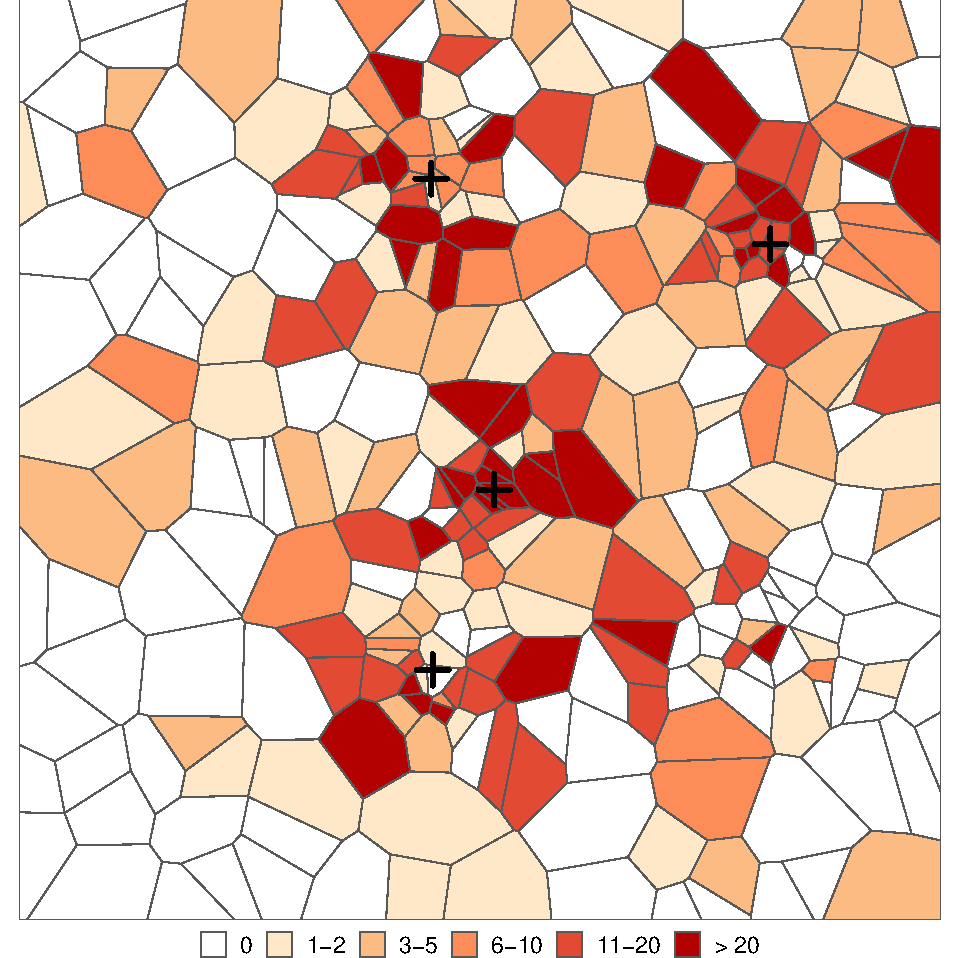
\includegraphics[width=0.8\textwidth]{figures/map_1_counts.pdf}}%
      \only<2>{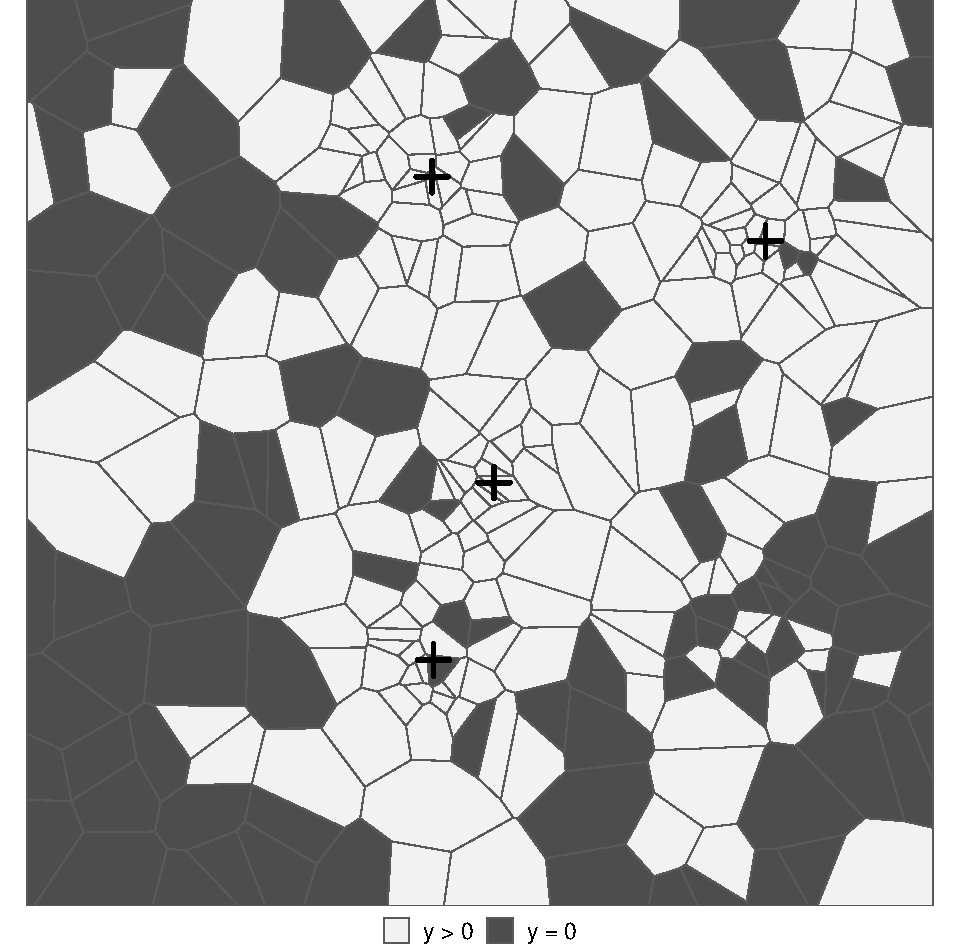
\includegraphics[width=0.8\textwidth]{figures/map_2_zeros.pdf}}%
      \only<3>{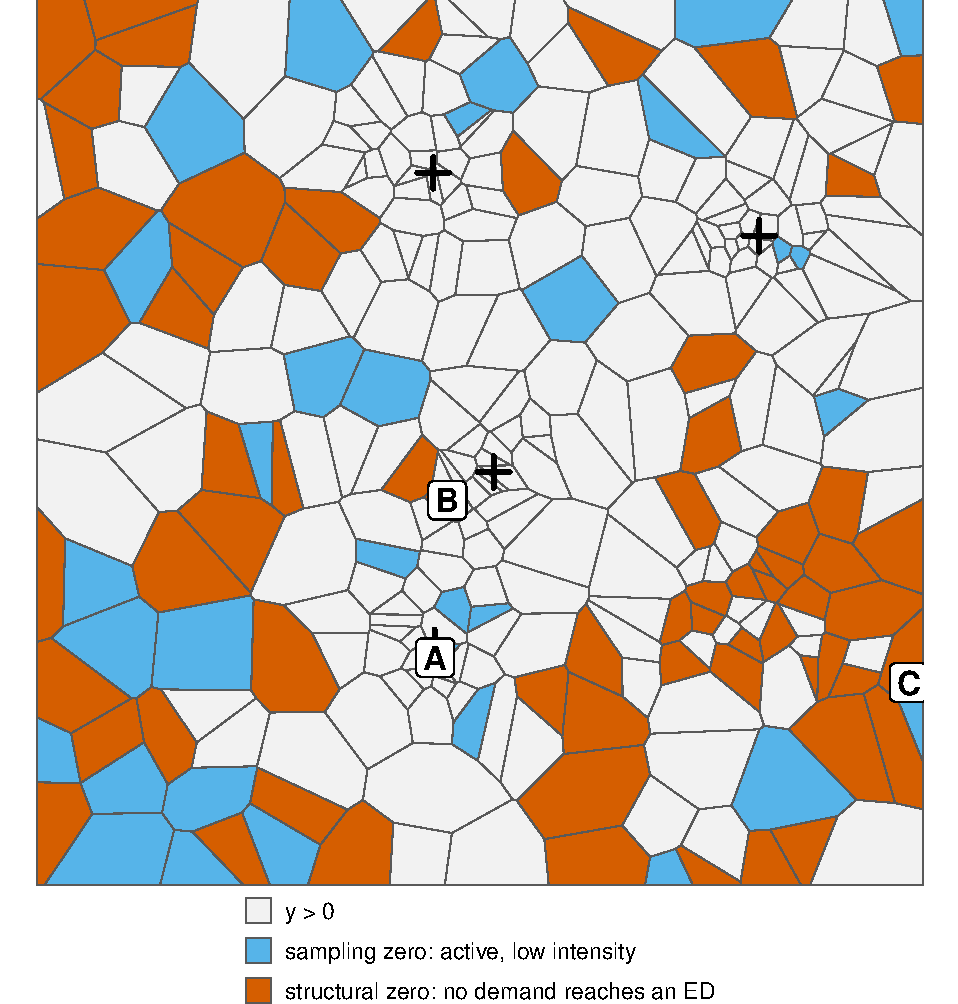
\includegraphics[width=0.8\textwidth]{figures/map_3_kinds.pdf}}%
      \only<4>{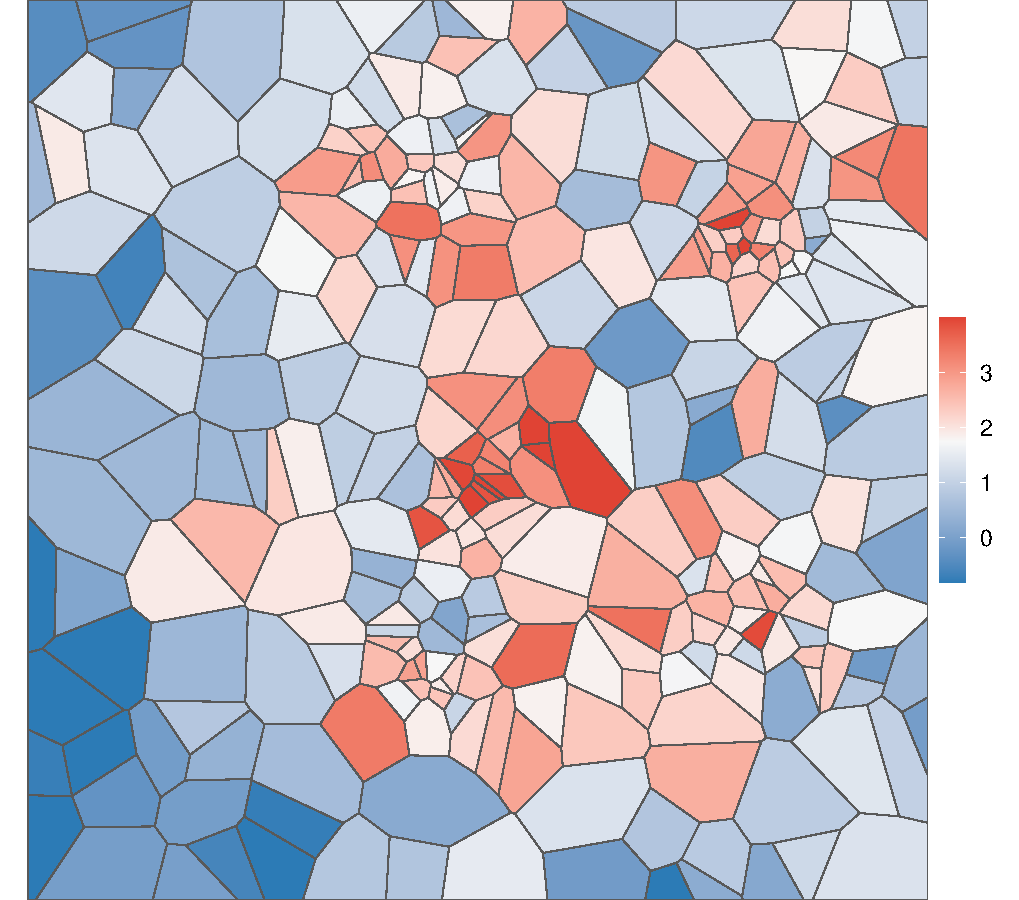
\includegraphics[width=0.8\textwidth]{figures/map_4_eta.pdf}}%
    \end{column}
    \begin{column}{0.44\textwidth}
      \vspace{1.5em}
      \only<1>{%
        \textbf{One municipality, one count.}\\[4pt]
        300 municipalities, the number of emergency-department visits in a period. Four hospitals with an ED, marked $+$.\\[8pt]
        Big counts around the hospitals, small counts in the periphery --- and a lot of white.\\[8pt]
        \textbf{What drives them:} population and distance to the nearest ED (and distance also drives the zeros). With real data: age structure, deprivation, GP supply.\\[8pt]
      }%
      \only<2>{%
        \textbf{Feature 1 --- many zeros.}\\[4pt]
        One municipality in three reports \emph{nothing}.\\[8pt]
        A Poisson with the right mean predicts almost none of them. A negative binomial can get there, but only by distorting every other parameter.\\[8pt]
        And the zeros are not scattered at random: they sit together.
      }%
      \only<3>{%
        \textbf{Feature 2 --- two kinds of zero.}\\[4pt]
        \footnotesize
        \textcolor{cyan!70!black}{\textbf{Sampling zero}}: the municipality is ``on'', but its risk is low and nothing happened this period.\\[2pt]
        \textbf{A} --- a small village of young families next to a hospital: nobody needed the ED this month; next month it may report two visits.\\[6pt]
        \textcolor{accent}{\textbf{Structural zero}}: no demand can reach these EDs.\\[2pt]
        \textbf{B} --- an industrial area or a nature reserve next to a hospital: almost nobody lives there.\\[2pt]
        \textbf{C} --- a border municipality: residents use the hospital of the next region, outside our data.\\[6pt]
        Same zero on the map; a different regime underneath.
      }%
      \only<4>{%
        \textbf{Feature 3 --- neighbours look alike.}\\[4pt]
        Behind every count there is an \emph{underlying risk} of using the ED (the model calls it the propensity $\eta_i$). Take away the zeros and the luck of the draw: this map is what is left.\\[8pt]
        Neighbouring municipalities have similar risk --- partly for observed reasons (population, distance), partly for unobserved ones: the same GP practice, the same habits, the same ambulance service.\\[8pt]
        ZISAR estimates this map; $\rho$ says how strongly a municipality's risk follows its neighbours'.
      }%
    \end{column}
  \end{columns}
\end{frame}

\begin{frame}{Three features, one signature}
  \begin{columns}[c]
    \begin{column}{0.62\textwidth}
      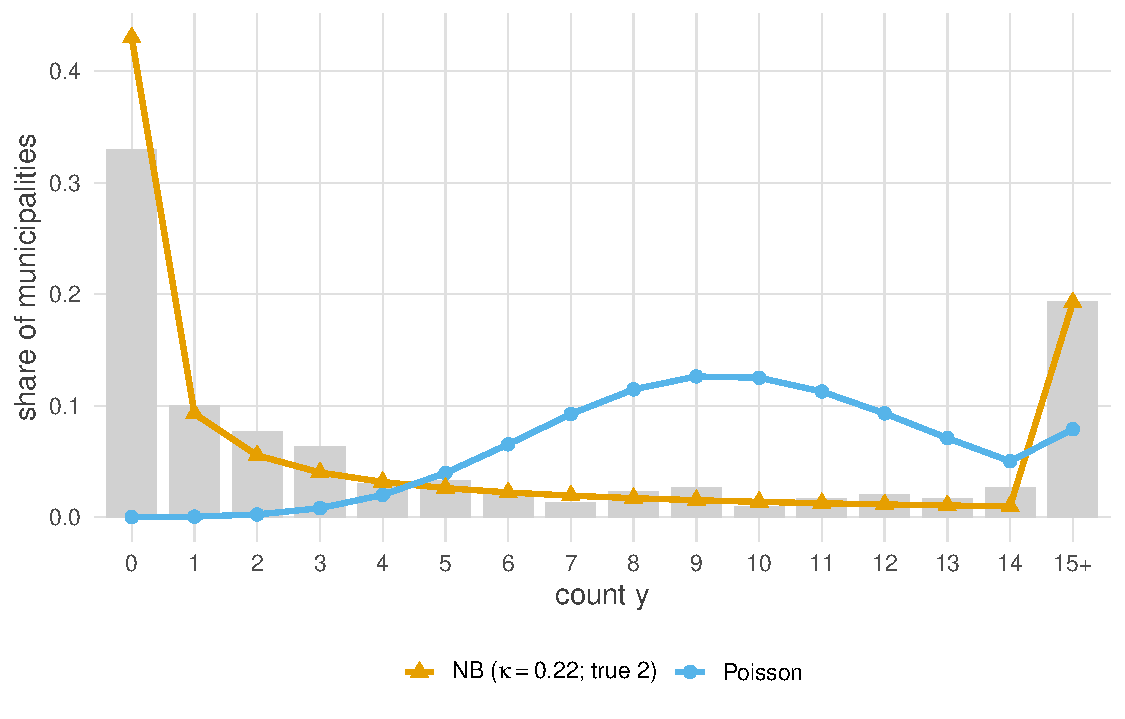
\includegraphics[width=\textwidth]{figures/fig_zeros.pdf}
    \end{column}
    \begin{column}{0.36\textwidth}
      {\color{accent}\large\bfseries 1}\quad{\bfseries Many zeros}\\
      {\small 33\% observed. A Poisson predicts none; an NB gets there (and beyond, 43\%) only with $\kappa=0.22$ (true 2). And \emph{two kinds}: sampling, structural.}\\[0.8em]
      {\color{accent}\large\bfseries 2}\quad{\bfseries Overdispersion}\\
      {\small variance $\gg$ mean among the non-zeros; a Poisson understates every standard error.}\\[0.8em]
      {\color{accent}\large\bfseries 3}\quad{\bfseries Spatial dependence}\\
      {\small neighbours look alike even after covariates.}
    \end{column}
  \end{columns}
\end{frame}

\begin{frame}{How a zero-inflated negative binomial works}
  \begin{columns}[c]
    \begin{column}{0.5\textwidth}
      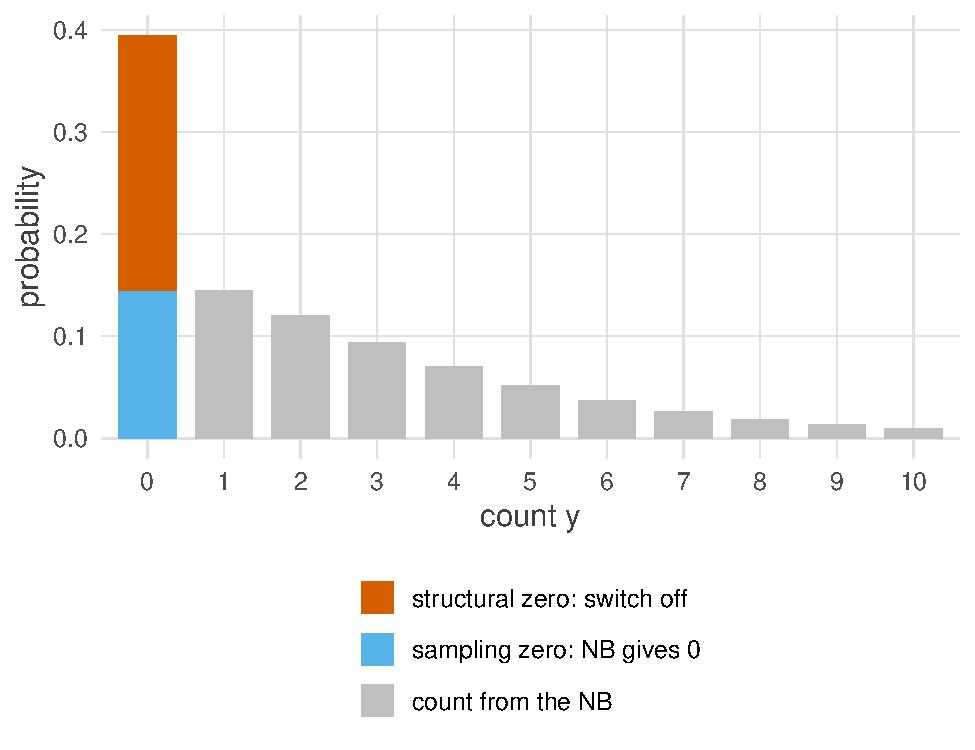
\includegraphics[width=\textwidth]{figures/fig_zinb.pdf}
    \end{column}
    \begin{column}{0.48\textwidth}
      \small
      \textbf{Two steps for each municipality}
      \begin{enumerate}\setlength{\itemsep}{0.15em}
        \item \textbf{A switch.} With probability $\pi_i$ the process is off: \textcolor{accent}{structural zero}.
        \item \textbf{A count.} Otherwise $y_i\sim\mathrm{NB}(\mu_i,\kappa)$, which can itself give a \textcolor{cyan!70!black}{sampling zero}.
      \end{enumerate}
      $P(y_i=0)=\pi_i+(1-\pi_i)\,\mathrm{NB}(0)$\\ $P(y_i=k)=(1-\pi_i)\,\mathrm{NB}(k)$\\[0.5em]
      \textbf{Two regressions}
      \begin{itemize}\setlength{\itemsep}{0.1em}
        \item $\logit\pi_i=\mathbf z_i'\bgamma$: who is switched off (distance to the ED).
        \item $\log\mu_i=\mathbf x_i'\bbeta$: how many visits when on (population).
        \item NB variance $\mu_i+\mu_i^2/\kappa$: small $\kappa$, more spread than a Poisson.
      \end{itemize}
    \end{column}
  \end{columns}
\end{frame}

% =============================================================================
\sect{2. Three toolkits that do not talk to each other}

\begin{frame}{Toolkit A --- spatial econometrics: the SAR model}
  \[
    \by = \rho\,\bW\by + \bX\bbeta + \boldsymbol{\varepsilon}
    \qquad\Longrightarrow\qquad
    \by = \underbrace{(\bI-\rho\bW)^{-1}}_{\bS(\rho)}(\bX\bbeta+\boldsymbol{\varepsilon})
  \]
  \begin{itemize}\setlength{\itemsep}{0.4em}
    \item Anselin (1988), Lee (2004), Kelejian--Prucha (1998, 99), LeSage--Pace (2009), Arbia (2006, 2024).
    \item $\rho$ is a \emph{structural} parameter: endogenous interaction, not residual correlation.
    \item $\bS(\rho)=\sum_s \rho^s\bW^s$ gives the \alert{direct / indirect / total effects} decomposition --- the object policy people actually want.
    \item Built for continuous $\by$. For counts the lag moves into the mean: on $\log\bmu$ (Lambert, Brown \& Florax 2010, two-step LIML) or on a latent Gaussian field (Liesenfeld, Richard \& Vogler 2016, likelihood by importance sampling). Both Poisson, neither handles excess zeros.
  \end{itemize}
\end{frame}

\begin{frame}{Toolkit B --- biostatistics: zero-inflated counts with spatial random effects}
  \[
    \logit(\pi_i) = \mathbf z_i'\bgamma + g_i, \qquad
    \log\mu_i = \mathbf x_i'\bbeta + v_i, \qquad (\mathbf g,\mathbf v)\ \text{CAR / Gaussian process}
  \]
  \begin{itemize}\setlength{\itemsep}{0.4em}
    \item Besag--York--Mollié (1991) random effects inside a ZIP/ZINB; \texttt{CARBayes} (Lee 2013), Neelon et al.\ (2013), INLA-based disease mapping, NNGP (He et al.\ 2024).
    \item Usually Bayesian; excellent at smoothing and mapping risk.
    \item Spatial dependence is a \alert{latent nuisance}, not an interaction: no $\rho$ with an interaction meaning, no indirect effects, no ``what happens in $i$ if I intervene in $j$''.
  \end{itemize}
\end{frame}

\begin{frame}{Toolkit C --- spatial filtering}
  \begin{itemize}\setlength{\itemsep}{0.8em}
    \item \textbf{Idea} (Griffith 2003): add to the regression a few ``map patterns'' --- eigenvectors of $\bW$ --- that soak up the spatial correlation, then fit any ordinary ZIP/ZINB.
    \item Used inside a zero-inflated model by Metulini, Patuelli \& Griffith (2018).
    \item Pragmatic and easy. But there is no $\rho$ and no spillover: space is \alert{removed}, not measured.
  \end{itemize}
\end{frame}

\begin{frame}{The gap}
  \centering
  \footnotesize
  \setlength{\tabcolsep}{4pt}
  \begin{tabular}{lccccc}
    \toprule
    Model & Spatial lag $\rho$ & Zero-infl. & Overdisp. & Heterog. & Spillovers \\
    \midrule
    SAR-Poisson (Lambert et al.\ 2010)      & \checkmark & -- & -- & -- & \checkmark \\
    SAL-Poisson (Liesenfeld et al.\ 2016)   & \checkmark & -- & -- & unit-level & \checkmark \\
    ZINB (Cameron--Trivedi 2013)             & -- & \checkmark & \checkmark & -- & -- \\
    ZIP + CAR (Lee 2013; Neelon et al.\ 2013) & -- & \checkmark & -- & CAR & -- \\
    ZINB + NNGP (He et al.\ 2024)           & -- & \checkmark & \checkmark & GP & -- \\
    ZIP + eigenvector filtering             & (proxy) & \checkmark & -- & -- & -- \\
    \midrule
    \color{accent}\textbf{ZISAR}            & \color{accent}\checkmark & \color{accent}\checkmark & \color{accent}\checkmark & \color{accent}unit-level & \color{accent}\checkmark \\
    \bottomrule
  \end{tabular}\\[1.5em]
  \normalsize
  \alert{What is new}: a structural $\rho$ inside a ZINB, a fast full likelihood (Laplace + TMB),\\ and evidence on what goes wrong without it.
\end{frame}

% =============================================================================
\sect{3. The ZISAR model}

\begin{frame}{The idea in one picture}
  \centering
  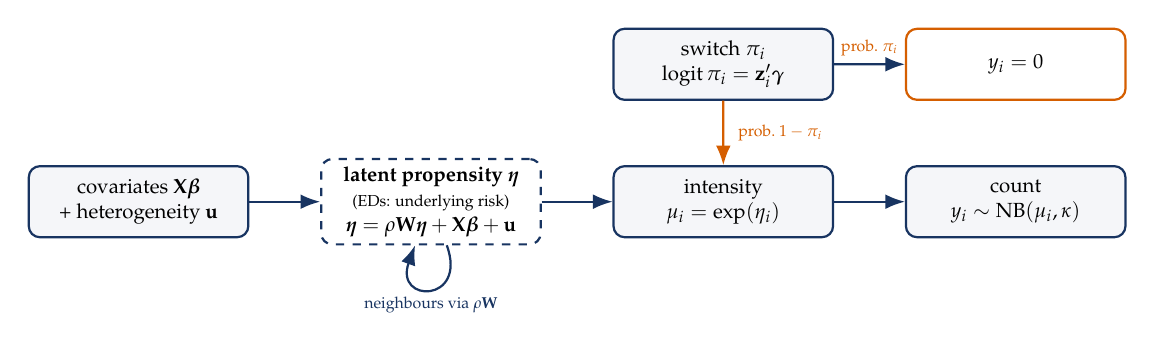
\begin{tikzpicture}[scale=0.82, transform shape,
      node distance=8mm and 11mm,
      box/.style={draw=navy,thick,rounded corners,fill=soft,minimum height=11mm,minimum width=34mm,align=center,font=\small},
      lat/.style={box,fill=white,dashed},
      arr/.style={-{Latex[length=2.5mm]},thick,navy}]
    \node[box] (X) {covariates $\bX\bbeta$\\+ heterogeneity $\bu$};
    \node[lat,right=of X] (eta) {\textbf{latent propensity} $\boldsymbol\eta$\\{\scriptsize (EDs: underlying risk)}\\$\boldsymbol\eta=\rho\bW\boldsymbol\eta+\bX\bbeta+\bu$};
    \node[box,right=of eta] (mu) {intensity\\$\mu_i=\exp(\eta_i)$};
    \node[box,right=of mu] (y) {count\\$y_i\sim\mathrm{NB}(\mu_i,\kappa)$};
    \node[box,above=of mu,yshift=2mm] (pi) {switch $\pi_i$\\$\logit\pi_i=\mathbf z_i'\bgamma$};
    \node[box,fill=white,draw=accent,right=of pi] (zero) {$y_i = 0$};
    \draw[arr] (X) -- (eta);
    \draw[arr] (eta) -- (mu);
    \draw[arr] (mu) -- (y);
    \draw[arr] (pi) -- node[above,font=\scriptsize,color=accent]{prob.\ $\pi_i$} (zero);
    \draw[arr,accent] (pi.south) -- node[right,font=\scriptsize,xshift=1mm]{prob.\ $1-\pi_i$} (mu.north);
    \draw[arr] (eta) edge[loop below,looseness=5,in=250,out=290,min distance=9mm] node[below,font=\scriptsize]{neighbours via $\rho\bW$} (eta);
  \end{tikzpicture}
  \vspace{0.8em}
  \begin{itemize}
    \item \textbf{In words:} each place has a latent propensity $\eta_i$ --- for EDs, its underlying risk of attendance. Propensities interact across neighbours \emph{before} they are turned into counts. On top, a switch can set the count to zero.
    \item \textbf{The design choice:} spatial feedback acts on $\boldsymbol\eta$, not on the observed $\by$.
  \end{itemize}
\end{frame}

\begin{frame}{Formally}
  \begin{align*}
    y_i &\sim \begin{cases} 0 & \text{w.p. } \pi_i \\ \mathrm{NB}(\mu_i,\kappa) & \text{w.p. } 1-\pi_i\end{cases}
    &&\text{\small $\Var[y_i\mid \text{count}] = \mu_i+\mu_i^2/\kappa$}\\[2pt]
    \mu_i &= \exp(\eta_i), \qquad
    \boldsymbol\eta = \rho\bW\boldsymbol\eta + \bX\bbeta + \bu, \quad \bu\sim N(\mathbf 0,\sigma^2\bI)
    &&\text{\small\alert{SAR on the latent predictor}}\\[2pt]
    \boldsymbol\eta &= \bS(\rho)\,(\bX\bbeta+\bu), \qquad \bS(\rho) = (\bI-\rho\bW)^{-1}
    &&\text{\small reduced form}\\[2pt]
    \logit(\pi_i) &= \mathbf z_i'\bgamma
    &&\text{\small the switch}
  \end{align*}
  \vspace{0.2em}
  Parameters: $\btheta = (\bbeta',\rho,\bgamma',\kappa,\sigma^2)'$.
  \vspace{0.4em}
  \begin{block}{Implied covariance of the latent field}
    $\Var[\boldsymbol\eta] = \sigma^2\,\bS(\rho)\bS(\rho)' = \sigma^2\big[(\bI-\rho\bW)'(\bI-\rho\bW)\big]^{-1}$ --- the SAR covariance of Anselin (1988), to be contrasted with the CAR precision $(\bI-\rho\bW)$ of disease mapping.
  \end{block}
\end{frame}

\begin{frame}{The switch has no space: what setting $g_i=0$ means}
  \small
  \[
    \logit(\pi_i) = \mathbf z_i'\bgamma + g_i, \qquad \mathbf g = (\bI-\rho_0\bW)^{-1}\boldsymbol\varepsilon_0
    \qquad\longrightarrow\qquad \text{today: } g_i = 0
  \]
  \begin{itemize}\setlength{\itemsep}{0.55em}
    \item \textbf{What it says.} Structural zeros cluster only as much as their covariates do. Two border villages are both switched off because both are far from an ED --- not because of each other.
    \item \textbf{What it rules out.} Zeros that cluster for reasons $\bZ$ does not see: a valley served by the hospital of the next region. If that happens, the model has one place to put the pattern --- low intensity in the count field --- so it can leak into $\hat\rho$ and into the split between structural and sampling zeros.
    \item \textbf{What it implies for effects.} Covariates in the switch act only locally: no spillover through the zeros.
    \item \textbf{Why we accept it.} The general model adds a second latent field of size $n$ and two parameters $(\rho_0,\sigma_0^2)$, and $\rho_0$ is learnt from the zeros alone: weakly identified unless they are many. Not yet in our code.
    \item \textbf{How to check it.} Choose $\bZ$ with a substantive story (distance, catchment), and look for clustering in the switch residuals. The general model is the next step.
  \end{itemize}
\end{frame}

\begin{frame}{Why SAR on $\boldsymbol\eta$ and not on $\by$?}
  \begin{columns}[T]
    \begin{column}{0.48\textwidth}
      \begin{block}{SAR on $\by$: ``my count depends on your count''}
        $\log\mu_i = \mathbf x_i'\bbeta + \rho\sum_j w_{ij}\,y_j + v_i$
        \begin{itemize}
          \item $y_j$ is on both sides $\Rightarrow$ endogenous
          \item counts have no reduced form $\Rightarrow$ instruments, no likelihood
        \end{itemize}
      \end{block}
    \end{column}
    \begin{column}{0.48\textwidth}
      \begin{block}{SAR on $\boldsymbol\eta$: ``my risk depends on your risk''}
        $\boldsymbol\eta = \rho\bW\boldsymbol\eta + \bX\bbeta + \bu$
        \begin{itemize}
          \item $\boldsymbol\eta = \bS(\rho)(\bX\bbeta+\bu)$ $\Rightarrow$ full likelihood, no instruments
          \item \alert{same} $\bS(\rho)$ $\Rightarrow$ same direct / indirect effects as the linear SAR
        \end{itemize}
      \end{block}
    \end{column}
  \end{columns}
  \vspace{1em}
  Lambert et al.\ (2010) and Liesenfeld et al.\ (2016) already put the lag here, for Poisson counts. ZISAR adds the zeros.
\end{frame}

\begin{frame}{What $\rho$ does: the spatial multiplier}
  \centering
  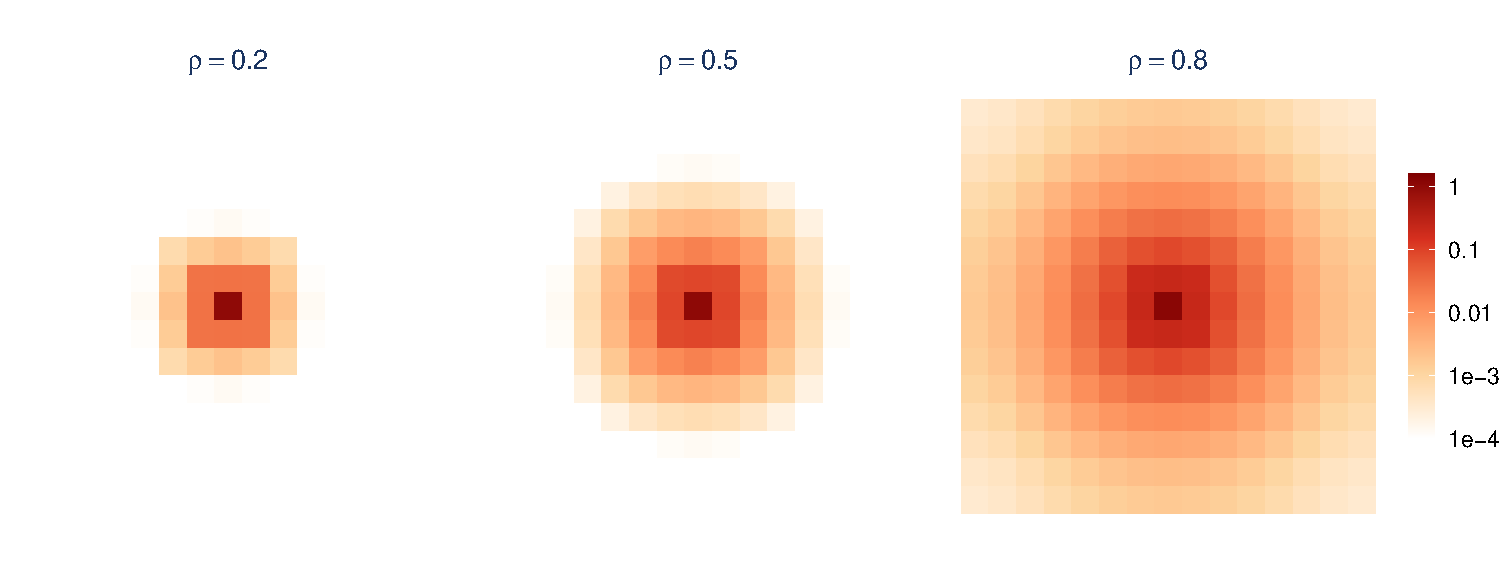
\includegraphics[width=0.78\textwidth]{figures/fig_multiplier.pdf}
  \vspace{0.3em}
  \begin{itemize}
    \item Something raises ED demand in the central municipality --- a care home opens, a GP practice closes. The colour is how much of that shock reaches each municipality around it (log scale).
    \item $\rho=0.2$: only the immediate neighbours feel it. $\rho=0.5$: three or four rings. $\rho=0.8$: the whole region.
    \item Mechanically, $\bS(\rho) = \bI + \rho\bW + \rho^2\bW^2 + \cdots$: neighbours, then neighbours of neighbours, each time weaker.
  \end{itemize}
\end{frame}

\begin{frame}{ZISAR contains its competitors}
  \centering
  \begin{tabular}{ll}
    \toprule
    Switch off & You get \\
    \midrule
    the zeros ($\pi_i=0$) & SAR-NB, a spatial negative binomial \\
    space ($\rho=0,\ \sigma^2=0$) & ZINB \\
    zeros and extra variance ($\pi_i=0,\ \kappa\to\infty,\ \sigma^2=0$) & SAR-Poisson (Lambert et al.\ 2010) \\
    everything & Poisson regression \\
    \bottomrule
  \end{tabular}
  \vspace{1.5em}
  \begin{itemize}
    \item So we can ask the data which pieces they need: fit with and without, and compare (a likelihood-ratio test).
  \end{itemize}
\end{frame}

% =============================================================================
\sect{4. Estimation}

\begin{frame}{The likelihood, and how we compute it}
  \[
    \ell(\btheta) = \log\int_{\mathbb R^n}
    \underbrace{\prod_{i=1}^n f(y_i\mid\eta_i,\pi_i;\kappa)}_{\text{ZINB for the counts}}\;
    \underbrace{p(\boldsymbol\eta\mid\bbeta,\rho,\sigma^2)}_{\text{SAR for the latent map}}\;
    \mathrm d\boldsymbol\eta
  \]
  \begin{itemize}
    \item In words: average the fit of the counts over every latent risk map the SAR finds plausible --- an integral in 300 dimensions, with no closed form.
  \end{itemize}
  \vspace{0.3em}
  \textbf{How: Laplace + TMB}
  \begin{enumerate}\setlength{\itemsep}{0.3em}
    \item For given parameters, find the most plausible latent map $\hat{\boldsymbol\eta}$. A few Newton steps, cheap because each municipality only talks to its 6 neighbours.
    \item Approximate the integral by a Gaussian centred there (Laplace approximation).
    \item TMB (Template Model Builder, Kristensen et al.\ 2016) computes all derivatives automatically; an optimiser adjusts the 8 parameters. \textbf{0.14\,s} for 300 municipalities.
  \end{enumerate}
  {\footnotesize Alternatives: MCMC (slow), importance sampling (Liesenfeld et al.), INLA (not built for a SAR with a free $\rho$).}
\end{frame}

\begin{frame}{Estimation on the map, step by step}
  \small
  \begin{columns}[T]
    \begin{column}{0.6\textwidth}
      \only<1>{\centering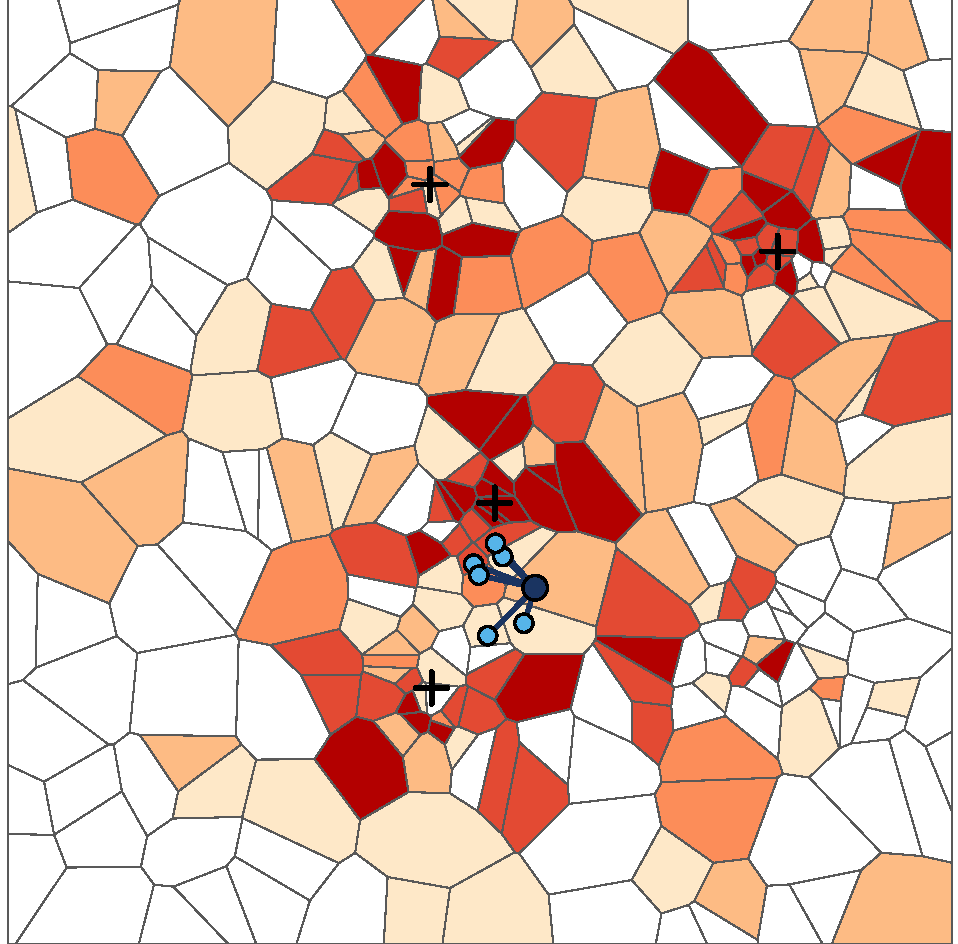
\includegraphics[width=0.74\textwidth]{figures/est_1_data.pdf}}%
      \only<2>{\centering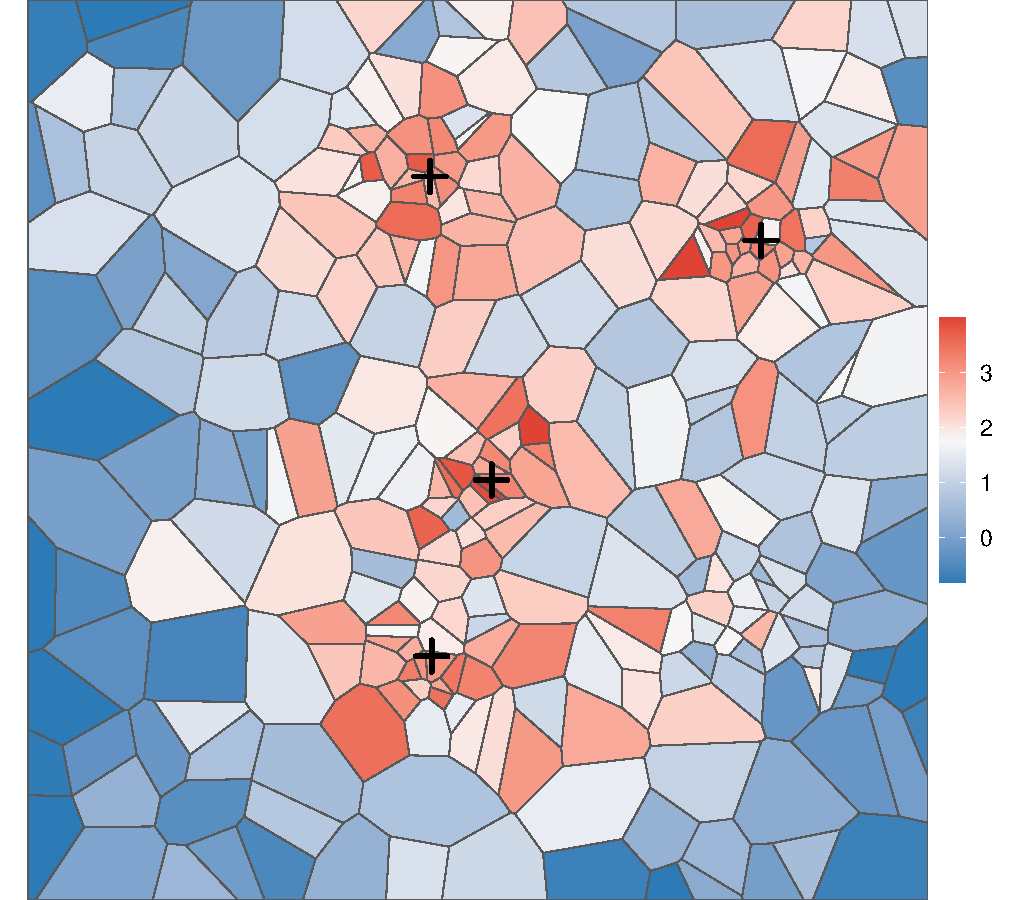
\includegraphics[width=0.8\textwidth]{figures/est_2_start.pdf}}%
      \only<3>{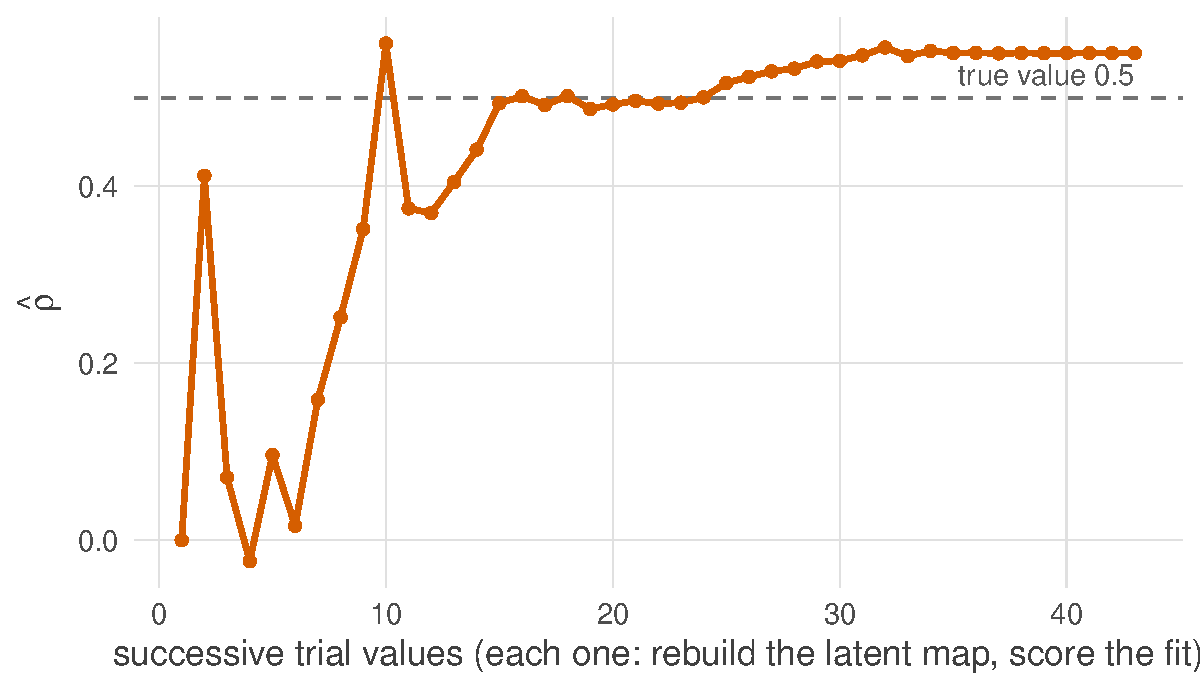
\includegraphics[width=\textwidth]{figures/est_4_outer.pdf}}%
      \only<4>{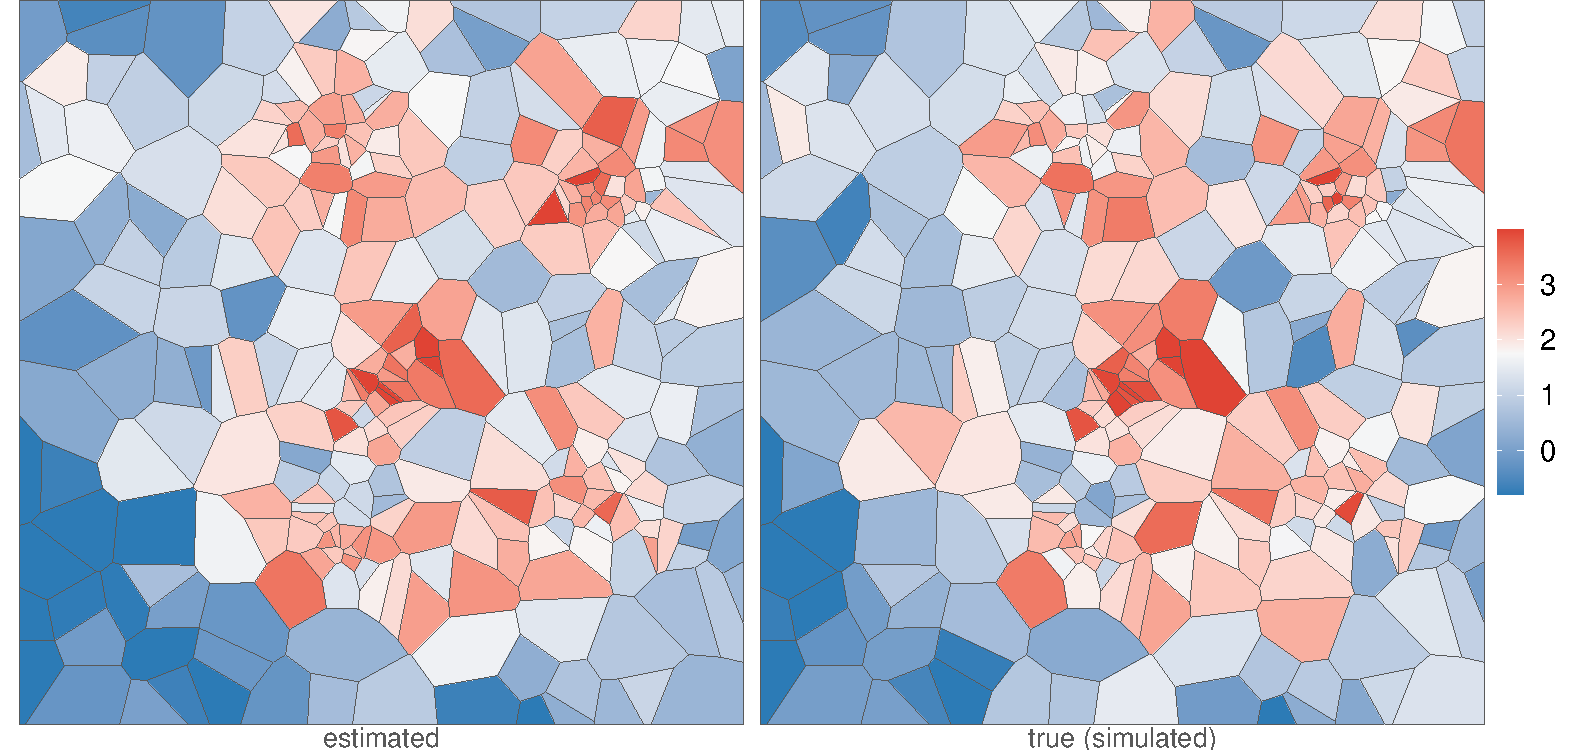
\includegraphics[width=\textwidth]{figures/est_5_result.pdf}}%
    \end{column}
    \begin{column}{0.4\textwidth}
      \vspace{0.5em}
      \only<1>{%
        \textbf{Step 0 --- the data.}\\[3pt]
        300 municipalities, 99 zeros (33\%), mean 9.9 visits, variance 456.\\[4pt]
        Covariates: population and distance to the nearest ED; distance also enters the switch.\\[4pt]
        Neighbours: the 6 nearest municipalities, each with weight $1/6$ (lines on the map).\\[4pt]
        Unknowns: 8 parameters ($\bbeta,\rho,\bgamma,\kappa,\sigma$) and the 300 latent risks $\eta_i$.
      }%
      \only<2>{%
        \textbf{Step 1 --- a starting guess.}\\[3pt]
        A plain Poisson regression on population and distance: the risk map the covariates alone can explain. No space, no zeros yet.\\[6pt]
        For comparison, an aspatial NB on the same data finds a distance effect of $-0.92$ (truth $-0.20$) and $\kappa=0.64$ (truth 2): it pushes the zeros and the clusters into the coefficients.
      }%
      \only<3>{%
        \textbf{Step 2 --- the search.}\\[3pt]
        The optimiser tries parameter values. For each trial it
        \begin{itemize}
          \item rebuilds the most plausible latent risk map: zeros pull a municipality down, large counts pull it up, neighbours pull each other together;
          \item scores how well that map explains the counts.
        \end{itemize}
        $\hat\rho$ starts at 0, overshoots, settles at 0.55.\\[4pt]
        34 iterations, \textbf{0.14\,s}. TMB supplies exact derivatives, so the search is short.
      }%
      \only<4>{%
        \textbf{Step 3 --- the result.}\\[3pt]
        \begin{tabular}{@{}lrrr@{}}
          & truth & est. & SE\\
          \midrule
          $\beta_{\text{population}}$ & 0.70 & 0.77 & 0.08\\
          $\beta_{\text{distance}}$ & $-0.20$ & $-0.19$ & 0.07\\
          $\rho$ & 0.50 & 0.55 & 0.08\\
          $\gamma_{\text{distance}}$ & 1.40 & 1.42 & 0.26\\
          $\kappa$ & 2.00 & 1.38 & 0.32\\
          $\sigma$ & 0.50 & 0.37 & 0.14\\
        \end{tabular}\\[5pt]
        Is there spatial dependence? Likelihood-ratio test of $\rho=0$: 18.5, $p\approx2\cdot10^{-5}$.\\
        Estimated vs true risk map: correlation 0.91.\\[4pt]
        {\footnotesize $\kappa$ and $\sigma$ both below truth: two ways of saying ``overdispersion'' that trade off --- the one weak spot in the Monte Carlo too.}
      }%
    \end{column}
  \end{columns}
\end{frame}

% =============================================================================
\sect{5. Does it work? Monte Carlo}

\begin{frame}{Design}
  \begin{columns}[T]
    \begin{column}{0.5\textwidth}
      \textbf{DGP} --- restricted ZISAR, queen contiguity on a square lattice
      \begin{itemize}
        \item $n\in\{100,225,400\}$, $\rho\in\{0,0.15,0.3,0.45,0.6\}$, $R=1000$ per cell
        \item $\bbeta=(0.5,0.8,-0.5)'$, $\bgamma=(-1,0.4)'$, $\kappa=2$, $\sigma=0.5$
        \item $\approx$ 40--50\% zeros, structural + sampling
      \end{itemize}
      \vspace{0.5em}
      \textbf{Competitors}
      \begin{itemize}
        \item \textcolor{orange!80!black}{\textbf{ZINB}} --- \texttt{pscl::zeroinfl}, ignores space
        \item \textcolor{cyan!70!black}{\textbf{SAR-NB}} --- NB GLM with instrumented $\widehat{\bW\by}$, $\bH=[\bX,\bW\bX,\bW^2\bX]$, ignores zeros
        \item \textcolor{accent}{\textbf{ZISAR}} --- TMB / Laplace
      \end{itemize}
      {\small The ZINB has no $\rho$: it assumes $\rho=0$, so in the $\hat\rho$ plots it sits on zero.}
    \end{column}
    \begin{column}{0.5\textwidth}
      \textbf{What we look at}
      \begin{itemize}
        \item the estimated $\hat\rho$ and $\hat\beta_1$ against the true values
        \item RMSE, convergence, seconds per fit
      \end{itemize}
      \vspace{0.5em}
      \begin{block}{The two questions}
        \begin{enumerate}
          \item What does ignoring zeros do to $\hat\rho$?
          \item What does ignoring space do to $\hat\bbeta$?
        \end{enumerate}
      \end{block}
    \end{column}
  \end{columns}
\end{frame}

\begin{frame}{Ignoring the zeros destroys $\hat\rho$ --- and $n$ does not help}
  \centering
  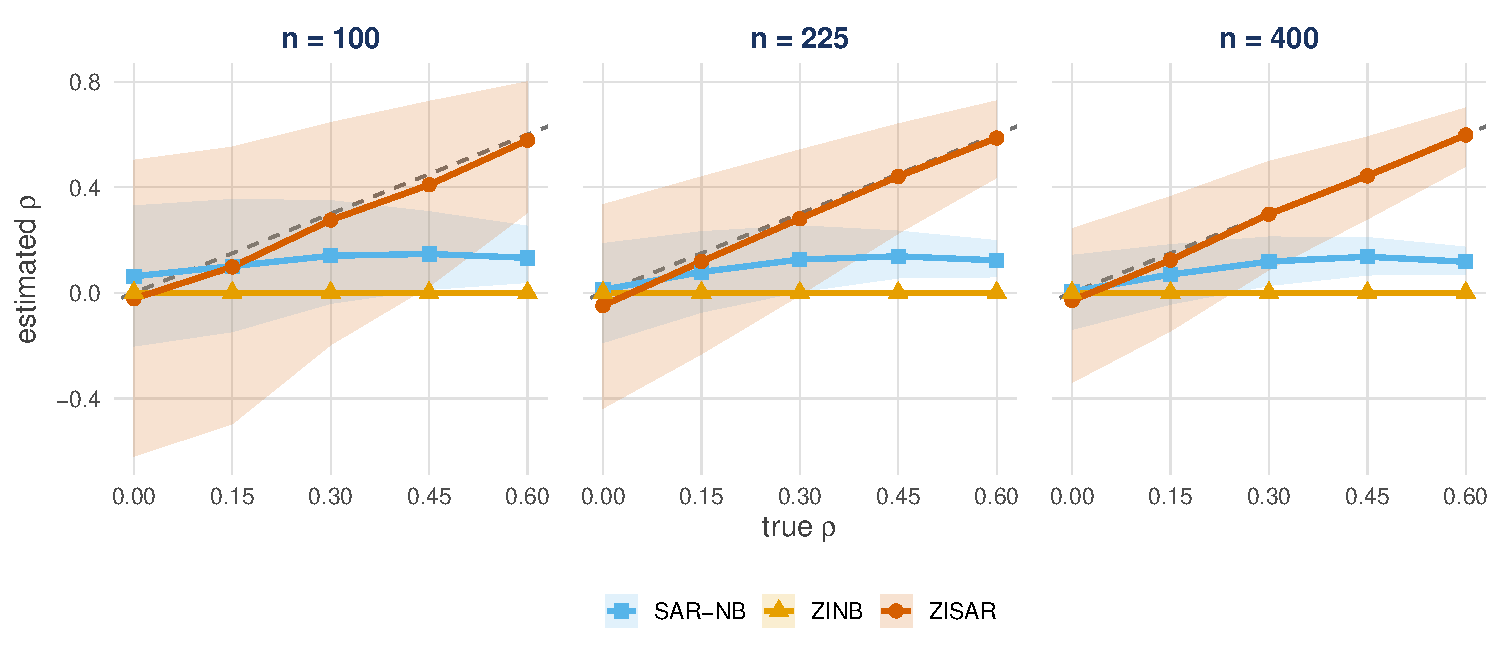
\includegraphics[width=0.78\textwidth]{figures/fig_mc_rho.pdf}
  \begin{itemize}\small
    \item Lines: average estimate over 1000 replications; bands: 10th--90th percentile; dashed: the truth. The ZINB sits at 0 by construction.
    \item SAR-NB flattens out: at $\rho_0=0.6$ it estimates 0.13, 0.12, 0.12 as $n$ grows. Not a small-sample problem: the model is wrong.
    \item ZISAR follows the diagonal (0.58, 0.59, 0.60 at $\rho_0=0.6$); its band is wide at $n=100$ and narrows fast.
  \end{itemize}
\end{frame}

\begin{frame}{Precision of $\hat\rho$}
  \centering
  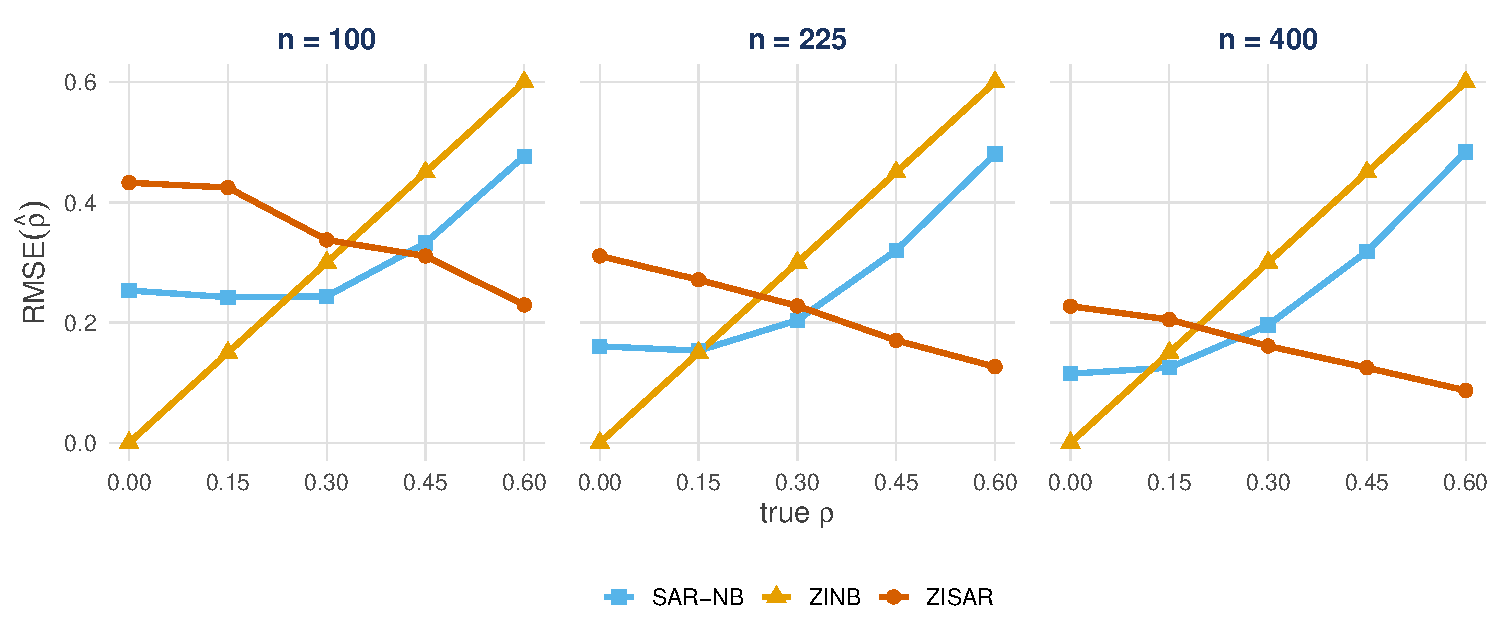
\includegraphics[width=0.74\textwidth]{figures/fig_mc_rho_rmse.pdf}
  \begin{itemize}\small
    \item At $\rho_0=0$ the SAR-NB is tighter (RMSE 0.12 vs 0.23 at $n=400$): with nothing to find, a simpler estimator wins. ZISAR pays for the extra variance component.
    \item From $\rho_0\approx0.3$ ($0.45$ at $n=100$) the ranking reverses, and the SAR-NB error is essentially its bias (0.48 at $\rho_0=0.6$, vs 0.09 for ZISAR).
    \item Honest note: 10\% of ZISAR fits (17\% at $n=100$) fail to converge or put $\hat\kappa$ at the boundary --- the $\kappa$ vs $\sigma^2$ trade-off --- and are excluded.
  \end{itemize}
\end{frame}

\begin{frame}{Ignoring space biases $\hat\bbeta$ and costs efficiency}
  \centering
  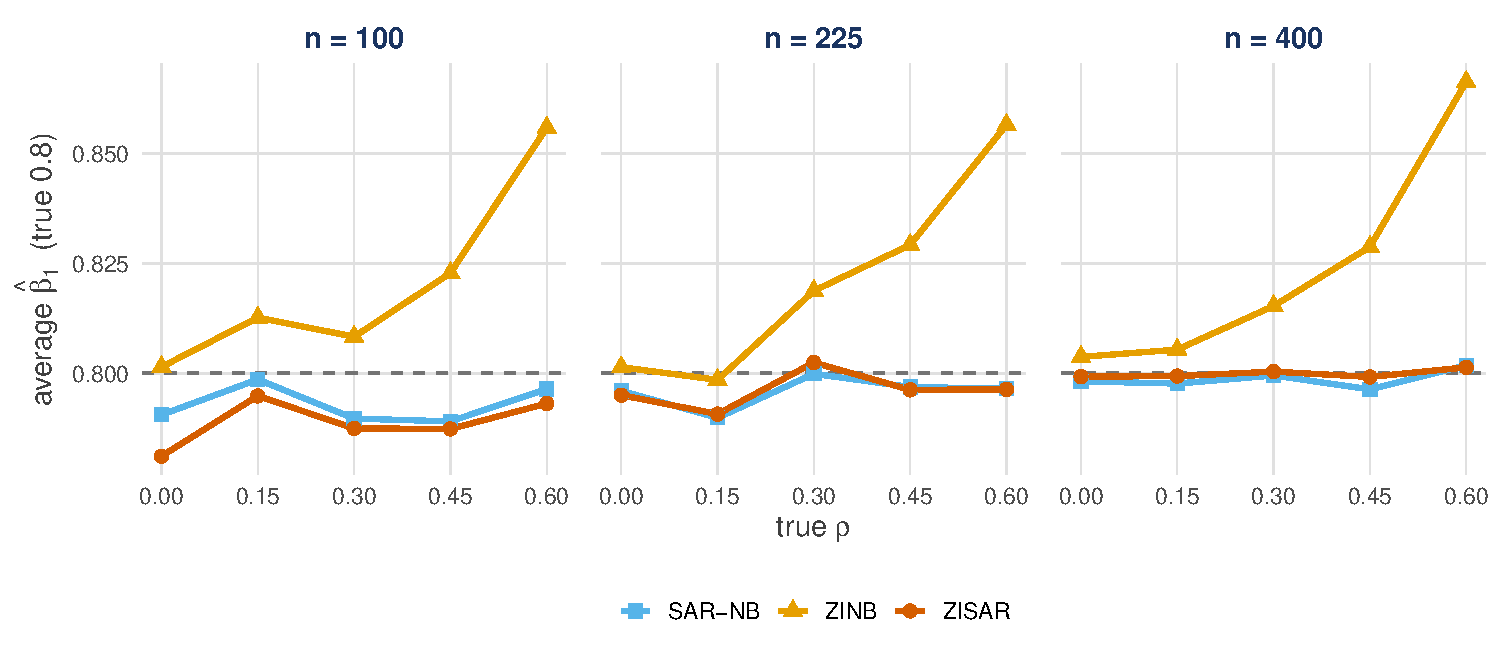
\includegraphics[width=0.82\textwidth]{figures/fig_mc_beta.pdf}
  \begin{itemize}\small
    \item The ZINB drifts away from 0.8 as $\rho_0$ grows ($+0.07$ at $\rho_0=0.6$), and more data do not help: the omitted spatial field ends up in the coefficient.
    \item ZISAR and SAR-NB stay on the truth. At $\rho_0=0.6$, $n=400$: RMSE$(\hat\beta_1)$ 0.079 ZISAR, 0.090 SAR-NB, 0.111 ZINB. At $\rho_0=0$ all three coincide.
  \end{itemize}
\end{frame}

% =============================================================================
\sect{6. Interpretation}

\begin{frame}{Coefficients are not effects: direct and indirect}
  \begin{columns}[c]
    \begin{column}{0.46\textwidth}
      \centering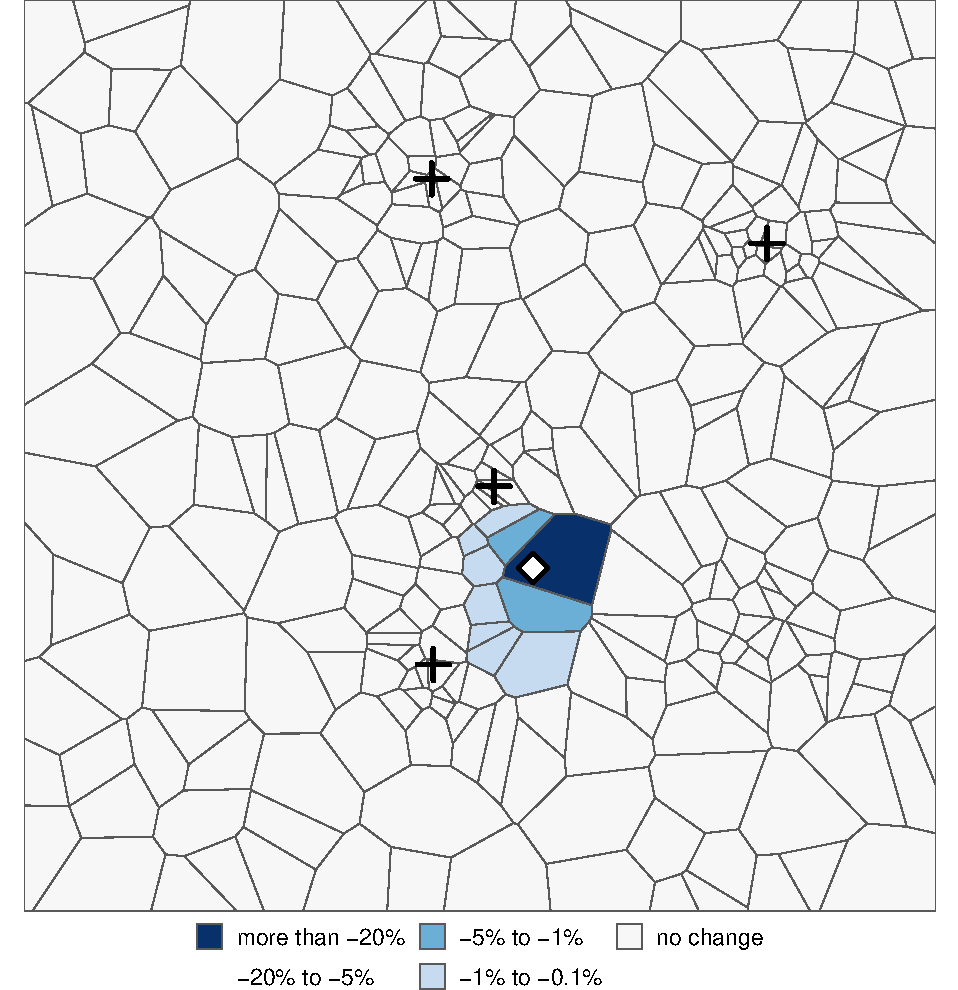
\includegraphics[width=0.92\textwidth]{figures/fig_effects_map.pdf}
    \end{column}
    \begin{column}{0.52\textwidth}
      An urgent-care clinic opens in the municipality marked $\diamond$; it lowers its ED risk ($\eta$) by 0.3. On the map of slide 5, with $\rho=0.5$:
      \begin{itemize}\setlength{\itemsep}{0.45em}
        \item \textbf{Direct effect}: $-1.6$ expected ED visits there ($-26\%$), including a small echo back from the neighbours.
        \item \textbf{Indirect effect} (spillover): $-0.7$ visits spread over 9 neighbouring municipalities, where nothing changed.
        \item \textbf{Total}: $-2.3$ visits for the region. A third of the effect happens next door.
      \end{itemize}
      \vspace{0.3em}
      A ZINB reports only the direct effect. Averaged over all municipalities, with $\rho=0.5$ the total is twice the direct.
    \end{column}
  \end{columns}
\end{frame}



% =============================================================================
\sect{7. Open problems}

\begin{frame}{What I would like to discuss with you}
  \small
  \begin{columns}[T]
    \begin{column}{0.5\textwidth}
      \textbf{Methodological}
      \begin{itemize}\setlength{\itemsep}{0.4em}
        \item Identification of $\rho$ vs $\rho_0$ in the general model (spatial switch): when do zeros carry their own spatial signal?
        \item $\sigma^2$ vs $\kappa^{-1}$: two ways to say ``overdispersion''; boundary estimates in 10--15\% of fits.
        \item Laplace accuracy with very sparse counts; higher-order corrections or importance sampling on top of TMB.
        \item $O(n^3)$ eigenvalues of $\bW$: stochastic log-determinants, or the pairwise/KD-tree ideas of Arbia--Nardelli--Salvini.
      \end{itemize}
    \end{column}
    \begin{column}{0.5\textwidth}
      \textbf{Extensions}
      \begin{itemize}\setlength{\itemsep}{0.4em}
        \item Space--time: $\eta_{it} = \rho(\bW\boldsymbol\eta_t)_i + \phi\,\eta_{i,t-1} + \mathbf x_{it}'\bbeta + u_i + \nu_t$.
        \item Several $\bW$'s (geographic, economic, network proximity) --- the ``relational'' side of territorial capital.
        \item Other count layers (CMP, generalised Poisson), other links for the switch.
        \item An \texttt{R} package with formula interface and \texttt{spdep}/\texttt{sf} integration.
      \end{itemize}
      \vspace{0.3em}
      \textbf{Applied}
      \begin{itemize}
        \item Which regional outcomes in your work look like this? Firm births, patents, migration flows at small scale?
      \end{itemize}
    \end{column}
  \end{columns}
\end{frame}

\begin{frame}{Limitations, stated plainly}
  \begin{enumerate}\setlength{\itemsep}{0.7em}
    \item \textbf{Asymptotics.} One latent $\eta_i$ per observation: the textbook $O(n^{-1})$ Laplace error is for a fixed number of random effects. Our consistency argument needs the approximation error to be negligible per unit; the SAR prior helps, but this is a condition we are still verifying. Today the evidence is the Monte Carlo.
    \item \textbf{Zeros vs.\ low intensity.} A zero can come from the switch or from a very low $\eta_i$; with a free $u_i$ per unit the switch is identified mainly through $\bZ$ and the functional form. Choose $\bZ$ with a substantive story.
    \item \textbf{$\kappa$ vs.\ $\sigma^2$.} Two ways of saying ``overdispersion''; in small samples the split is weakly identified (10--15\% of Monte Carlo fits at the boundary).
    \item \textbf{Competitors and data.} The Monte Carlo does not yet include a Bayesian CAR competitor nor ZISAR with $\pi=0$; the application still runs on synthetic data, real data next (York).
  \end{enumerate}
\end{frame}

\begin{frame}{Take-aways}
  \begin{enumerate}\setlength{\itemsep}{0.7em}
    \item Spatial counts with excess zeros need \alert{both} a switch and a spatial interaction; existing tools give you one or the other.
    \item Putting the SAR on the \alert{latent propensity} keeps the econometric meaning of $\rho$ and the effects decomposition, and makes maximum likelihood feasible.
    \item Laplace + automatic differentiation turns an $n$-dimensional integral into a one-second fit.
    \item Ignoring zeros flattens $\hat\rho$ (0.12 when the truth is 0.6) and more data do not help; ignoring space biases $\hat\bbeta$ and reports zero spillovers.
  \end{enumerate}
  \vspace{1em}
  \centering
  {\large Thank you.}\\[4pt]
  {\small niccolo.salvini@unicatt.it}
\end{frame}

% =============================================================================
\appendix
\sect{Backup}

\begin{frame}{Backup: illustrative application on a Piedmont-like region}
  \footnotesize
  \begin{columns}[T]
    \begin{column}{0.5\textwidth}
      \textbf{Setting}
      \begin{itemize}
        \item $n=300$ municipalities, all-cause ED visits in one period (synthetic, Piedmont-like)
        \item 25\% zeros; mean 6.1, variance 81
        \item $\bW$: 6 nearest neighbours, row-standardised
      \end{itemize}
      \vspace{0.2em}
      \textbf{Count $\bX$}: log-population, aging index, distance to nearest ED, income\\[2pt]
      \textbf{Switch $\bZ$}: distance to nearest ED, GP density\\[4pt]
      {\color{navy}\textbf{Why these two.}} A structural zero is ``no demand reaches this ED'': distance, and GPs that absorb demand.
    \end{column}
    \begin{column}{0.5\textwidth}
      \textbf{What the synthetic run shows} {\scriptsize(truth: $\rho=0.35$, $\kappa=2$)}
      \begin{itemize}\setlength{\itemsep}{0.25em}
        \item \textbf{ZISAR}: $\hat\rho=0.41$ (SE 0.15), $\hat\kappa=2.03$, $\hat\sigma=0.39$; every $\hat\beta$ within one SE of the truth.
        \item \textbf{SAR-NB} (no zeros): the distance effect vanishes ($-0.03$ vs.\ $0.20$) and $\hat\kappa=0.69$: the zeros become overdispersion.
        \item \textbf{ZINB} (no space): slopes close, but the intercept absorbs the multiplier (1.92 vs.\ 1.20) and $\hat\kappa=1.33$.
        \item Indirect $\approx40\%$ of total, imprecise at $n=300$.
        \item Moran's $I$ $\approx0$ and n.s.\ on all three residuals --- and on $\by$ itself ($0.02$, $p=0.24$). With zeros and overdispersion a residual test misses a dependence the likelihood estimates at $\hat\rho=0.41$.
      \end{itemize}
      \vspace{0.1em}
      \begin{block}{Next: real data}
        April--May 2027, \alert{CHE York}, with Rita Santos: ED attendances by small area (slide 2).
      \end{block}
    \end{column}
  \end{columns}
\end{frame}

\begin{frame}{Backup: the effects decomposition, formally}
  \small
  Change covariate $r$ in unit $j$; the response of $\E[\by]$ in every unit $i$ is the $n\times n$ matrix
  \[
    \mathbf M_r = \diag\!\big((\mathbf 1-\hat\bpi)\odot\hat\bmu\big)\;\bS(\rho)\;\beta_r
    \;+\;
    \underbrace{\big[-\diag(\hat\bmu)\diag(\hat\bpi\odot(\mathbf 1-\hat\bpi))\,\gamma_r\big]}_{\text{inflation channel, diagonal if } r\in\bZ}
  \]
  \[
    \overline M_r^{\text{direct}} = n^{-1}\tr\mathbf M_r,\qquad
    \overline M_r^{\text{total}} = n^{-1}\mathbf 1'\mathbf M_r\mathbf 1,\qquad
    \overline M_r^{\text{indirect}} = \text{total}-\text{direct}.
  \]
  \begin{columns}[T]
    \begin{column}{0.5\textwidth}
      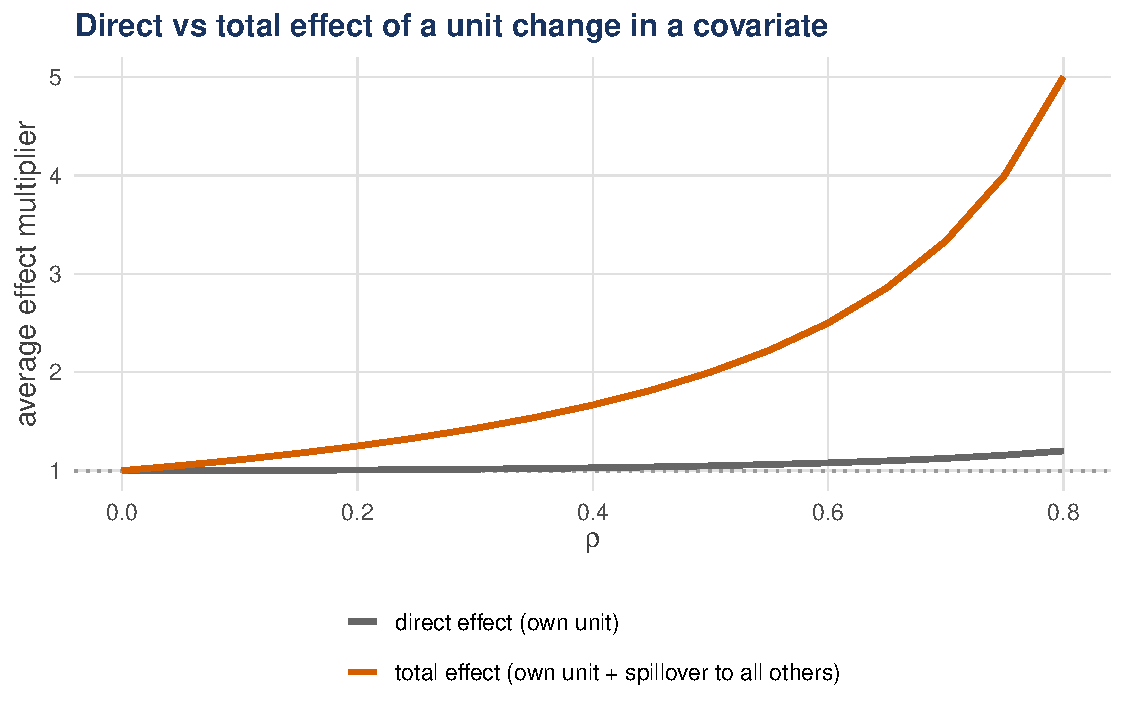
\includegraphics[width=0.95\textwidth]{figures/fig_effects.pdf}
    \end{column}
    \begin{column}{0.5\textwidth}
      \vspace{0.5em}
      \begin{itemize}\setlength{\itemsep}{0.4em}
        \item LeSage--Pace (2009) scaled by the ZINB mean $(1-\pi_i)\mu_i$.
        \item Indirect effect $=0$ \emph{iff} $\rho=0$; sign of $\beta_r$ preserved; monotone in $|\rho|$.
        \item SEs by simulating $\btheta^{(b)}\sim N(\hat\btheta,\hat{\mathbf V})$, $B=500$.
        \item A ZINB reports zero spillover by construction.
      \end{itemize}
    \end{column}
  \end{columns}
\end{frame}

\begin{frame}{Backup: asymptotics (the short version)}
  \begin{block}{Assumptions}
    (W) $\bW_n$ uniformly bounded in row/column sums, $\rho$ in a compact subset of $(-1/r_{\max},1/r_{\max})$;
    (X) exogenous regressors with $n^{-1}\bX'\bX\to\mathbf Q_X>0$;
    (P) true $\btheta_0$ interior, $\kappa_0,\sigma_0^2>0$;
    (I) $\E[\ell(\btheta)]$ uniquely maximised at $\btheta_0$.
  \end{block}
  \vspace{0.5em}
  \begin{itemize}\setlength{\itemsep}{0.5em}
    \item \textbf{Consistency.} Laplace error is $O(n^{-1})$ (Tierney--Kadane 1986), so $n^{-1}\ell_{\mathrm{LA}}\to n^{-1}\ell$ uniformly; standard extremum-estimator argument (Newey--McFadden 1994).
    \item \textbf{Asymptotic normality.} $\sqrt n(\hat\btheta_n-\btheta_0)\xrightarrow{d}N(\mathbf 0,\mathcal I(\btheta_0)^{-1})$ by mean-value expansion of the score and a CLT for spatially dependent arrays under (W) --- the Lee (2004) route.
    \item \textbf{Honest caveat.} The Laplace approximation is a first-order approximation to a non-Gaussian integral; with very sparse counts and many zeros its accuracy is the thing to check (we do, in the Monte Carlo).
  \end{itemize}
\end{frame}


\begin{frame}{Backup: overdispersion attribution, fit and speed ($R=100$)}
  \centering
  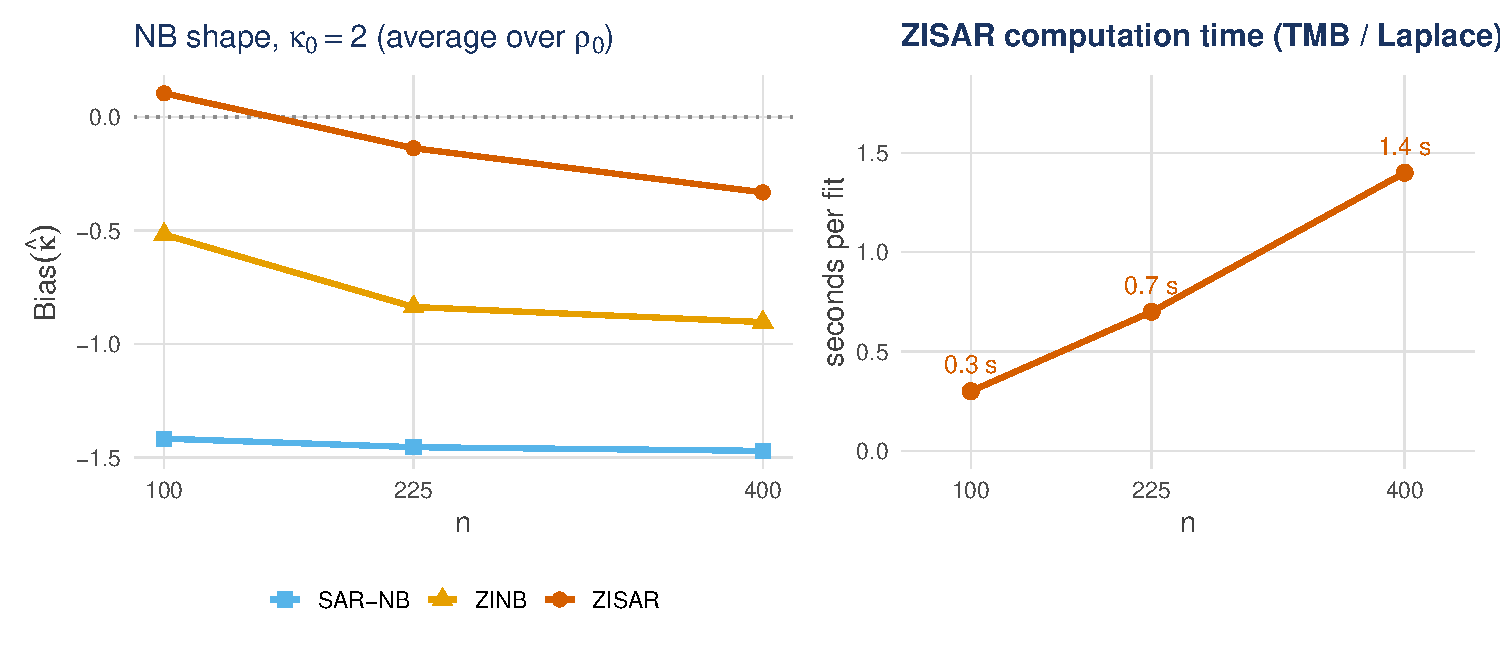
\includegraphics[width=0.7\textwidth]{figures/fig_mc_kappa_time.pdf}
  \begin{itemize}\small
    \item Both competitors push $\kappa$ down (``more overdispersion'') to explain zeros and clusters they do not model; SAR-NB is off by $-1.4$ on a true value of 2.
    \item Median log-likelihood: ZISAR best whenever $\rho_0>0$, gap over ZINB growing with $\rho_0$ and $n$ (15 nats at $n=400$, $\rho_0=0.6$: $-869$ vs $-884$); indistinguishable at $\rho_0=0$.
    \item Convergence 96--100\%; 10--15\% of fits hit the $\kappa$ boundary (the classic $\sigma^2$ vs $\kappa^{-1}$ trade-off) and are flagged.
  \end{itemize}
\end{frame}


\begin{frame}{Backup: the estimation algorithm}
  \small
  \begin{enumerate}\setlength{\itemsep}{0.3em}
    \item \textbf{Pre-compute} eigenvalues of $\bW$; sparse Cholesky ordering of $(\bI-\rho\bW)'(\bI-\rho\bW)$.
    \item \textbf{Initialise} $\bbeta^{(0)}$ from a Poisson GLM, $\bgamma^{(0)}=(\logit(\text{share of zeros}),0,\dots)$, $\rho=0$, $\kappa=1$, $\sigma=0.5$; $\boldsymbol\eta^{(0)}=\bX\bbeta^{(0)}$.
    \item \textbf{Objective}: $f(\boldsymbol\eta;\btheta) = -\sum_i\log f(y_i\mid\eta_i,\pi_i;\kappa) - \log p(\boldsymbol\eta\mid\bbeta,\rho,\sigma^2)$, with $\boldsymbol\eta$ declared as random effects in TMB.
    \item \textbf{Repeat}: inner Newton--Raphson for $\hat{\boldsymbol\eta}(\btheta^{(s)})$ with sparse Cholesky; evaluate $\ell_{\mathrm{LA}}$ and $\nabla_{\btheta}\ell_{\mathrm{LA}}$ by AD; \texttt{nlminb} step on $\btheta$.
    \item \textbf{Output}: $\hat\btheta$, AD Hessian $\Rightarrow\hat{\mathbf V}$, delta-method SEs on the original scale (\texttt{sdreport}).
  \end{enumerate}
  \vspace{0.5em}
  \textbf{ZINB pmf with mean $e^\eta$ and shape $\kappa$}
  \[
    f(y\mid\eta,\pi;\kappa)=
    \begin{cases}
      \pi + (1-\pi)\,h(0;\eta,\kappa) & y=0\\
      (1-\pi)\,h(y;\eta,\kappa) & y\ge 1
    \end{cases}
  \]
  \[
    h(y;\eta,\kappa)=\frac{\Gamma(y+\kappa)}{\Gamma(\kappa)\Gamma(y+1)}\Big(\frac{\kappa}{\kappa+e^\eta}\Big)^{\kappa}\Big(\frac{e^\eta}{\kappa+e^\eta}\Big)^{y}.
  \]
\end{frame}

\begin{frame}{Backup: spatial dependence is not just a nuisance}
  \begin{columns}[T]
    \begin{column}{0.55\textwidth}
      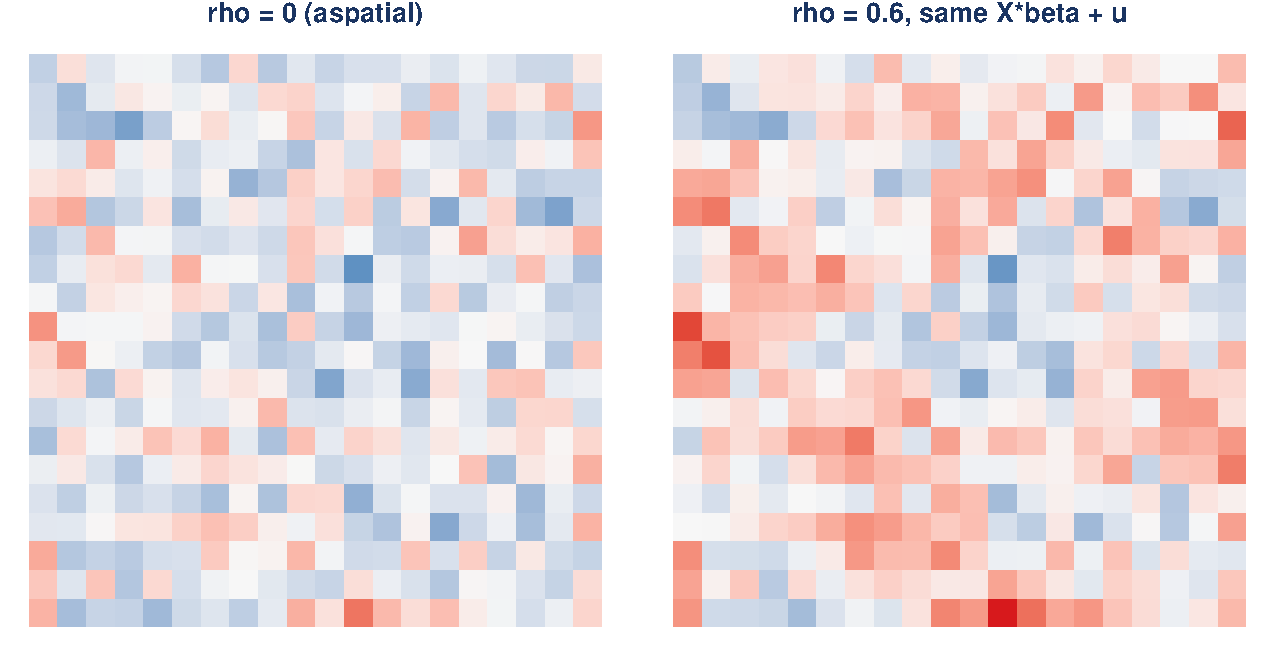
\includegraphics[width=\textwidth]{figures/fig_lattice.pdf}
    \end{column}
    \begin{column}{0.45\textwidth}
      Same covariates, same unobserved heterogeneity. The only difference is a feedback parameter $\rho$.
      \vspace{0.6em}
      \begin{itemize}\setlength{\itemsep}{0.4em}
        \item Left: what an aspatial model assumes.
        \item Right: what a spatial-lag model generates --- clusters that are \emph{not} in $\bX$.
        \item An aspatial regression on the right panel attributes the clusters to whatever covariate happens to be clustered too.
      \end{itemize}
      \vspace{0.6em}
      {\small This is the mechanism behind the bias we will see in the Monte Carlo.}
    \end{column}
  \end{columns}
\end{frame}


\begin{frame}{Backup: zero-inflation or hurdle?}
  \small
  \begin{columns}[T]
    \begin{column}{0.5\textwidth}
      \textbf{Zero-inflated (ZISAR)}
      \[
        P(y{=}0) = \pi + (1-\pi)h(0),\quad P(y{=}k) = (1-\pi)h(k)
      \]
      \begin{itemize}
        \item two sources of zeros, mixed: a unit can be ``on'' and still record zero
        \item the switch and the count share the zeros, so $\pi$ and $\mu$ are identified jointly through the covariates and the spatial structure
        \item natural when the structural zero is a latent state (no at-risk population, demand served elsewhere)
      \end{itemize}
    \end{column}
    \begin{column}{0.5\textwidth}
      \textbf{Hurdle (Neelon et al.\ 2013)}
      \[
        P(y{=}0) = \pi,\quad P(y{=}k) = (1-\pi)\,\tfrac{h(k)}{1-h(0)}
      \]
      \begin{itemize}
        \item all zeros from the first stage; the count is truncated at zero
        \item two likelihoods that separate cleanly --- simpler, but the count process no longer ``owns'' any zero
        \item natural when zero is an observed decision (participate / not)
      \end{itemize}
    \end{column}
  \end{columns}
  \vspace{0.3em}
  \begin{block}{In the TMB template}
    The hurdle version changes the observation block only; latent field, Laplace step and effects are unchanged. Both can be fitted and compared by AIC/BIC on the same data.
  \end{block}
\end{frame}

\begin{frame}{Backup: three channels of overdispersion, and how they are told apart}
  \small
  Marginal variance of $y_i$ (integrating the latent field), with $\E[\mu_i] = \exp\!\bigl(\bar\eta_i + \tfrac12\sigma^2[\bS\bS']_{ii}\bigr)$:
  \[
    \Var[y_i] = (1-\pi_i)\,\E[\mu_i]\bigl(1+\kappa^{-1}\E[\mu_i]\bigr) + \pi_i(1-\pi_i)\,\E[\mu_i]^2 + (1-\pi_i)\,\Var[\mu_i]
  \]
  \begin{itemize}\setlength{\itemsep}{0.4em}
    \item \textbf{$\kappa$ (NB shape)}: extra variance \emph{within} a unit, proportional to $\mu_i^2$, no spatial pattern.
    \item \textbf{$\pi_i$ (zeros)}: extra variance from the mixture, tied to $\bZ$ and to the share of zeros.
    \item \textbf{$\sigma^2$ (heterogeneity)}: extra variance \emph{between} units, amplified by $[\bS(\rho)\bS(\rho)']_{ii}$ --- so it is spatially patterned when $\rho\neq0$.
  \end{itemize}
  \vspace{0.4em}
  \begin{block}{Identification in practice}
    $\kappa$ and $\sigma^2$ are separated by the \emph{shape} of the extra variance (quadratic in $\mu$ vs log-normal) and by its spatial structure; $\pi_i$ by the excess at zero. Where the data are too sparse to separate $\kappa$ from $\sigma^2$, the fit drifts to the $\kappa$ boundary --- the 10--15\% of Monte Carlo replications we flag. A profile likelihood in $\log\kappa$ makes this visible for a given dataset.
  \end{block}
\end{frame}

\begin{frame}{Backup: how good is the Laplace approximation here?}
  \small
  \begin{itemize}\setlength{\itemsep}{0.45em}
    \item The integrand in $\boldsymbol\eta$ is a Gaussian SAR prior times a product of ZINB terms; each term is log-concave in $\eta_i$ for $y_i\geq1$, and for $y_i=0$ it is bounded and smooth. The conditional mode is unique in all our fits.
    \item Laplace is exact for Gaussian observation models and has error $O(n^{-1})$ in the marginal likelihood (Tierney--Kadane 1986); the practical risk is \emph{skewness} of $p(\eta_i\mid y_i)$ when $y_i=0$ and $\pi_i$ is large.
    \item \textbf{Checks we can run on any dataset:} (i) importance sampling around the Laplace mode (TMB: \texttt{MCMC} / \texttt{tmbstan} for a Hamiltonian check); (ii) refit with the restricted vs general switch; (iii) compare with \texttt{glmmTMB} ZINB + i.i.d.\ RE at $\rho=0$, which uses the same approximation.
    \item \textbf{Monte Carlo evidence:} bias of $\hat\rho$ and $\hat\bbeta$ is negligible at $n\geq225$ with 40--50\% zeros, which is the regime where the approximation would be expected to struggle.
    \item Where it is not enough: higher-order Laplace (Shun--McCullagh), or INLA-style numerical integration over the few hyper-parameters with Laplace only for the latent field.
  \end{itemize}
\end{frame}

\begin{frame}{Backup: SAR on $\boldsymbol\eta$ vs CAR --- what is the difference in practice?}
  \small
  \begin{columns}[T]
    \begin{column}{0.5\textwidth}
      \textbf{SAR (ZISAR)}
      \[
        \Var[\boldsymbol\eta] = \sigma^2\bigl[(\bI-\rho\bW)'(\bI-\rho\bW)\bigr]^{-1}
      \]
      \begin{itemize}
        \item precision is quadratic in $\bW$: second-order neighbours enter
        \item $\rho$ is the coefficient of a simultaneous equation --- an interaction
        \item effects: $\partial\E[\by]/\partial x_{jr}$ via $\bS(\rho)$, so a shock in $j$ reaches every $i$
        \item the mean $\bS(\rho)\bX\bbeta$ is spatially multiplied too
      \end{itemize}
    \end{column}
    \begin{column}{0.5\textwidth}
      \textbf{CAR (BYM, CARBayes)}
      \[
        \Var[\boldsymbol\eta] = \sigma^2\bigl(\mathbf D-\rho\bW\bigr)^{-1}
      \]
      \begin{itemize}
        \item precision is linear in $\bW$: only first-order neighbours
        \item $\rho$ is a smoothing parameter of a conditional prior
        \item the mean is $\bX\bbeta$ unchanged: covariates do not spill over
        \item usually symmetric $\bW$ required; row-standardised $\bW$ needs the Leroux/proper-CAR variant
      \end{itemize}
    \end{column}
  \end{columns}
  \vspace{0.5em}
  {\small Both are Gaussian Markov random fields; the SAR is the one whose parameter has an econometric reading. In the TMB template, swapping the prior block gives the CAR version of the same zero-inflated model, which is a useful robustness check.}
\end{frame}

\begin{frame}{Backup: choosing $\bW$, and what the diagnostics look like}
  \small
  \begin{itemize}\setlength{\itemsep}{0.45em}
    \item \textbf{Candidates for municipalities:} queen contiguity; $k$-nearest neighbours ($k=4,6,8$) on centroids; inverse-distance with a cut-off; travel-time to the nearest ED. Row-standardised so that $\rho\in(-1,1)$ and $\bW\boldsymbol\eta$ is a neighbourhood average.
    \item \textbf{Selection:} fit each, compare marginal log-likelihood / AIC (the $\log\det$ term is already in the likelihood, so this is legitimate); report $\hat\rho$ under all of them --- the sign and significance should be stable, the magnitude will not be (it scales with the density of $\bW$).
    \item \textbf{Residual diagnostics:} Moran's $I$ on Pearson residuals $(y_i-\hat{\E}[y_i])/\sqrt{\widehat{\Var}[y_i]}$ under the chosen $\bW$ \emph{and} under the alternatives; randomised quantile residuals for the count layer; observed vs predicted share of zeros by neighbourhood.
    \item \textbf{In the synthetic Piedmont run:} Moran's $I$ is $\approx0$ and not significant on all three models' residuals and on $\by$ itself ($0.02$, $p=0.24$), while ZISAR estimates $\hat\rho=0.41$ (SE 0.15): with zeros and overdispersion, residual tests have little power --- use the likelihood (LR on $\rho$) as the main diagnostic.
    \item \textbf{Endogenous $\bW$} (e.g.\ patient flows) is a different model: it is on the extensions list, not in the current estimator.
  \end{itemize}
\end{frame}

\begin{frame}{Backup: computational cost and scaling}
  \begin{center}
    \footnotesize
    \begin{tabular}{p{3.2cm} p{3cm} p{7.2cm}}
      \toprule
      Step & Cost & Notes \\
      \midrule
      Eigenvalues of $\bW$ (once) & $O(n^3)$ dense & only step that does not scale; replace with Barry--Pace (1999) MC estimator or Chebyshev approximation \\
      Inner Newton step & $O(n)$--$O(n^{3/2})$ & sparse Cholesky of $\bH$, fill-in depends on ordering (nested dissection for lattices) \\
      $\log\det\bH$ & free & from the Cholesky factor \\
      AD gradient of $\ell_{\mathrm{LA}}$ & $\approx$ 2--4$\times$ one evaluation & reverse-mode AD through inner and outer problem \\
      Outer \texttt{nlminb} & 30--40 iterations & 34 iterations on the 300-unit map, starting from a Poisson GLM \\
      \bottomrule
    \end{tabular}
  \end{center}
  \vspace{0.4em}
  \begin{itemize}
    \item Measured: 0.3\,s ($n=100$), 0.7\,s ($n=225$), 1.4\,s ($n=400$) per fit, single core, including \texttt{sdreport}.
    \item Not yet benchmarked beyond $n=400$: the dense eigendecomposition is the first step to break as $n$ grows; with a sparse $\log\det$ the rest scales with the Cholesky fill-in.
    \item The Monte Carlo: $9$ scenarios $\times$ $100$ replications $\times$ $3$ models.
  \end{itemize}
\end{frame}

\begin{frame}{Backup: the general model with a spatial switch}
  \small
  \[
    \logit(\pi_i) = \mathbf z_i'\bgamma + g_i, \qquad \mathbf g = (\bI-\rho_0\bW)^{-1}\boldsymbol\varepsilon_0, \quad \boldsymbol\varepsilon_0\sim N(\mathbf 0,\sigma_0^2\bI)
  \]
  \begin{itemize}\setlength{\itemsep}{0.45em}
    \item \textbf{Why one might want it:} structural zeros cluster for their own reasons --- a whole valley served by one hospital across the border, an area with no at-risk population. Then the switch is spatially organised independently of the count intensity.
    \item \textbf{What it costs:} a second latent field of dimension $n$ in the Laplace approximation (same sparse machinery, roughly $2\times$ the cost), and two more parameters $(\rho_0,\sigma_0^2)$.
    \item \textbf{Identification:} $\rho_0$ is identified only through the zeros, so it needs many of them and enough covariate variation in $\bZ$; with 25\% zeros and $n=300$ the profile likelihood in $\rho_0$ is flat. With a shared field ($g_i\propto u_i$) identification is cleaner but the interpretation changes.
    \item \textbf{Effects:} the inflation channel of $\mathbf M_r$ is no longer diagonal, so covariates in $\bZ$ also produce indirect effects.
    \item \textbf{Our position:} the restricted model is the workhorse; the general one is a sensitivity check and a likelihood-ratio test of ``do the zeros cluster beyond what $\bZ$ explains?''
  \end{itemize}
\end{frame}

\begin{frame}{Backup: the space--time extension}
  \[
    \eta_{it} = \rho\,(\bW\boldsymbol\eta_t)_i + \phi\,\eta_{i,t-1} + \mathbf x_{it}'\bbeta + u_i + \nu_t, \qquad y_{it}\sim \text{ZINB}(\pi_{it},\,e^{\eta_{it}},\,\kappa)
  \]
  \begin{itemize}\setlength{\itemsep}{0.45em}
    \item Same construction: a latent Gaussian field, now of dimension $nT$, with a sparse precision (block-tridiagonal in time, $\bW$-sparse in space); TMB handles it with the same Laplace step.
    \item Stationarity requires $|\rho|+|\phi|<1$ (for row-standardised $\bW$); the long-run multiplier becomes $(\bI-\rho\bW-\phi\bI)^{-1}$, and effects split into short-run and long-run, direct and indirect.
    \item The unit effect $u_i$ is now identified from the within-unit variation, which weakens the $\kappa$--$\sigma^2$ trade-off considerably.
    \item Open: initial conditions for $\eta_{i0}$; dynamic spatial panel asymptotics with fixed $T$; and whether the switch should have its own persistence.
    \item Natural datasets: monthly ED visits by municipality, yearly firm births by local labour market.
  \end{itemize}
\end{frame}

\begin{frame}{Backup: can a residual Moran test see the dependence?}
  \small
  \centering
  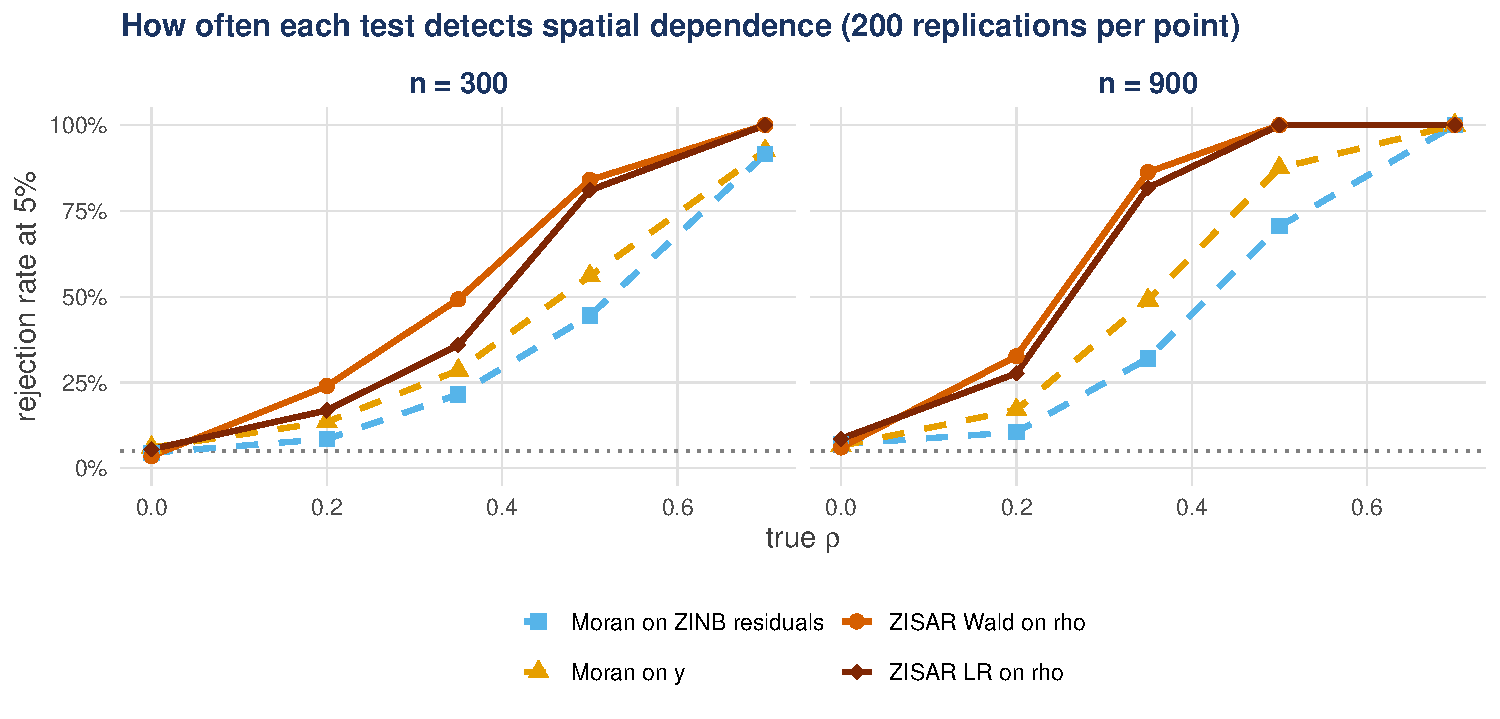
\includegraphics[width=0.7\textwidth]{figures/fig_power_moran.pdf}
  \begin{itemize}\setlength{\itemsep}{0.2em}
    \item Same design as the application (6-NN, 25--35\% zeros, $\kappa=2$), 200 datasets per point, ZINB and ZISAR fitted on each.
    \item At $\rho=0.35$, $n=300$: Moran on ZINB residuals detects it 22\% of the time, the ZISAR Wald test 49\%. At $n=900$: 32\% vs.\ 86\%.
    \item Under $\rho=0$ all tests are close to 5\%; the LR test is slightly liberal at $n=900$ (8.6\%).
  \end{itemize}
\end{frame}

\begin{frame}{Backup: Monte Carlo tables}
  \tiny
  \setlength{\tabcolsep}{3.5pt}
  \textbf{Bias of $\hat\rho$ (RMSE in parentheses), $R=100$}\\[3pt]
  \begin{tabular}{l rrr rrr rrr}
    \toprule
    & \multicolumn{3}{c}{$\rho_0=0$} & \multicolumn{3}{c}{$\rho_0=0.3$} & \multicolumn{3}{c}{$\rho_0=0.6$}\\
    \cmidrule(lr){2-4}\cmidrule(lr){5-7}\cmidrule(lr){8-10}
    & 100 & 225 & 400 & 100 & 225 & 400 & 100 & 225 & 400\\
    \midrule
    SAR-NB & 0.066 (.24) & $-$0.006 (.17) & 0.018 (.11) & $-$0.170 (.26) & $-$0.180 (.20) & $-$0.184 (.20) & $-$0.464 (.47) & $-$0.474 (.48) & $-$0.479 (.48)\\
    ZISAR  & $-$0.019 (.39) & $-$0.037 (.34) & $-$0.015 (.23) & $-$0.105 (.42) & $-$0.032 (.20) & 0.002 (.15) & $-$0.062 (.28) & $-$0.000 (.12) & $-$0.007 (.09)\\
    \bottomrule
  \end{tabular}
  \vspace{0.8em}

  \textbf{Bias of $\hat\beta_1$ ($\beta_1^0=0.8$) and median log-likelihood}\\[3pt]
  \begin{tabular}{ll rrr rrr rrr}
    \toprule
    & & \multicolumn{3}{c}{$\rho_0=0$} & \multicolumn{3}{c}{$\rho_0=0.3$} & \multicolumn{3}{c}{$\rho_0=0.6$}\\
    \cmidrule(lr){3-5}\cmidrule(lr){6-8}\cmidrule(lr){9-11}
    & & 100 & 225 & 400 & 100 & 225 & 400 & 100 & 225 & 400\\
    \midrule
    \multirow{3}{*}{Bias $\hat\beta_1$} & ZINB & 0.018 & $-$0.009 & 0.006 & $-$0.003 & $-$0.000 & 0.009 & 0.053 & 0.059 & 0.055\\
    & SAR-NB & 0.009 & $-$0.017 & 0.004 & $-$0.018 & $-$0.011 & $-$0.009 & 0.016 & 0.002 & 0.000\\
    & ZISAR & $-$0.012 & $-$0.014 & 0.008 & $-$0.020 & $-$0.008 & $-$0.003 & 0.011 & $-$0.002 & $-$0.002\\
    \midrule
    \multirow{3}{*}{Median $\ell$} & ZINB & $-$161 & $-$363 & $-$648 & $-$176 & $-$399 & $-$716 & $-$221 & $-$494 & $-$884\\
    & SAR-NB & $-$162 & $-$367 & $-$655 & $-$178 & $-$402 & $-$720 & $-$224 & $-$495 & $-$887\\
    & ZISAR & $-$160 & $-$363 & $-$648 & $-$175 & $-$396 & $-$713 & $-$218 & $-$486 & $-$869\\
    \bottomrule
  \end{tabular}
\end{frame}

\begin{frame}{Backup: selected references}
  \tiny
  \begin{itemize}\setlength{\itemsep}{0.15em}
    \item Anselin, L. (1988). \emph{Spatial Econometrics: Methods and Models}. Kluwer.
    \item Arbia, G. (2006). \emph{Spatial Econometrics}. Springer; Arbia, G. (2024). \emph{Spatial Econometrics} (2nd ed.).
    \item Arbia, G., Nardelli, V. (2024); Arbia, Nardelli, Salvini --- pairwise pseudo-likelihood and KD-tree sampling for large spatial models.
    \item Besag, J., York, J., Mollié, A. (1991). Bayesian image restoration with two applications in spatial statistics. \emph{Ann.\ Inst.\ Stat.\ Math.}
    \item Cameron, A.C., Trivedi, P.K. (2013). \emph{Regression Analysis of Count Data} (2nd ed.). CUP.
    \item Glaser, S. (2017). A review of spatial econometric models for count data. Hohenheim Discussion Papers.
    \item Kristensen, K., Nielsen, A., Berg, C.W., Skaug, H., Bell, B. (2016). TMB: Automatic differentiation and Laplace approximation. \emph{J.\ Stat.\ Software}.
    \item Lambert, D. (1992). Zero-inflated Poisson regression. \emph{Technometrics}.
    \item Lambert, D.M., Brown, J.P., Florax, R.J.G.M. (2010). A two-step estimator for a spatial lag model of counts. \emph{Reg.\ Sci.\ Urban Econ.}
    \item Lee, D. (2013). CARBayes. \emph{J.\ Stat.\ Software}; Lee, L.-F. (2004). Asymptotic distributions of QML estimators for spatial autoregressive models. \emph{Econometrica}.
    \item LeSage, J., Pace, R.K. (2009). \emph{Introduction to Spatial Econometrics}. CRC.
    \item Liesenfeld, R., Richard, J.-F., Vogler, J. (2016). Likelihood evaluation of high-dimensional spatial latent Gaussian models with non-Gaussian response variables. \emph{Advances in Econometrics} 37.
    \item Metulini, R., Patuelli, R., Griffith, D.A. (2018). A spatial-filtering zero-inflated approach to the estimation of the gravity model of trade. \emph{Econometrics}.
    \item Neelon, B., Ghosh, P., Loebs, P.F. (2013). A spatial Poisson hurdle model for exploring geographic variation in emergency department visits. \emph{JRSS-A}.
    \item Rue, H., Martino, S., Chopin, N. (2009). Approximate Bayesian inference for latent Gaussian models (INLA). \emph{JRSS-B}.
    \item Tierney, L., Kadane, J.B. (1986). Accurate approximations for posterior moments and marginal densities. \emph{JASA}.
  \end{itemize}
\end{frame}

\end{document}
